\documentclass[10pt,a4paper]{article}
\usepackage[utf8]{inputenc}
\usepackage[english]{babel}
\usepackage[T1]{fontenc}
\usepackage{amsmath}
\usepackage{amsfonts}
\usepackage{amssymb}
\usepackage{subcaption}
\usepackage{makeidx}
\usepackage{graphicx}
\usepackage{fourier}
\usepackage{listings}
\usepackage{color}
\usepackage{hyperref}
\usepackage[left=2cm,right=2cm,top=2cm,bottom=2cm]{geometry}
\author{Sigve Harang, Lukas Powalla}
\title{Space Physics Project , FYS3610}
\graphicspath{{./data/}} %BEEEEE CAREFUL WITH THIS LINE
\lstset{language=C++,
	keywordstyle=\bfseries\color{blue},
	commentstyle=\itshape\color{red},
	stringstyle=\color{green},
	identifierstyle=\bfseries,
	frame=single}
\begin{document}
\maketitle
\newpage
\tableofcontents
\newpage
\section*{Introduction}
In this project we are going to analyse the ionospheric and auroral dynamics and its relation to the solar wind conditions. 
The two most relevant physical mechanisms are magnetic reconnection and frozen in magnetic fields. We will also investigate the Earth's currentsystem. Magnetic fields and 
currentflows are governed by Magnethydrodynamics, and coupled trough Maxwell's equations. Finally, we will compare our observations to theory. 
We will investigate in a specific timeslot of 6 hours from the 6. January 2011 from 18:00 UT to the 07. January 2011 00:00 UT. We will not go into a detailed mathematical
description of the different phenomena, but we will provide a clear overview of a few aspects of the ionospheric and auroral dynamics.
\section{Theory part} 
In order to understand the movements and changes in the system of the earth and the sun, we want to introduce some basic concepts of space physics.
A really important steady state picture is the Dungey cycle. It tries to explain what is going on with respect to Earth's magnetic field, the interaction of Earth's
magnetic field with the Interplanetary Magnetic Field (hereafter IMF) and the current flow. The most important precondition for the Dungey cycle is that the IMF is orientated southward. The Dungey cycle is as already mentioned a steady state picture. This means that the magnetic flux added to the open magnetic field lines through dayside reconnection is equal to the magnetic flux subtracting from the open magnetic field lines through nightside reconnection. However, this model does not fully resolve ionospheric and auroral dynamics at small timescales. 
(by small timescales we mean compared to the full cycle). We observe different phases such as adding magnetic flux (growing of the polar cap), some kind of explosive expansion 
(subtraction of magnetic flux from the polar cap) and a recovery phase. This phenomena is called a "Auroral substorm". In addition to that, we can extract information 
about what is going on with Earth environment by looking at different data sets containing information about the magnetic field on Earth, the solar wind bulk speed, 
the auroral intensity, the current density and further data from different physical measurements. Based on these measurements we will interpret the received data and relate 
it to the theoretical predictions and the models we introduced in the theory part. The natural coordinate system is the GSM-system, but there is not much difference with respect to GSE. Both coordinate systems are good enough for our purpose. 
We don't want to include in this theory part how the discrete, diffuse or cusp aurora in particular works. However, if you want to investigate more in different types of aurora and how the are build, please have a look at chapter "14, THE AURORA AND THE AURORAL IONOSPHERE " in book \cite{Buch2}[p.459-502]. 

\subsection{The Dungey cycle - a steady state picture \label{_CHAP_THEO_Dungey cycle}}

\begin{figure}[h]
\centering
\caption{Dungey cycle; numbers belong to the description in section \ref{_CHAP_THEO_Dungey cycle}; the dashed line is the magneto-pause; full lines describe magnetic field lines}
\label{Dungey cycle}
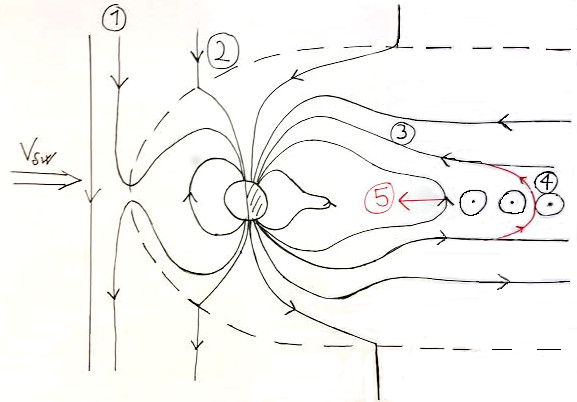
\includegraphics[scale=0.5]{solvind.jpg}
\end{figure}
If the magnetic field is northward orientated ($B_z>0$ in GSM/(GSE)-coordinates) then there is no magnetic reconnection on the dayside. 
The IMF can not mix with the terrestrial magnetic field because everything is frozen in. The solar wind will be deflected slightly and flow around the Earth, and stretch far into space anti-sunward. As long as the magnetic field of Earth and the IMF have magnetic field lines which have parallel orientation.  
Then, everything stays frozen in and the field lines must simply follow the IMF flow past the Earth. However, if the IMF is southward orientated ($B_z<0$), we have anti-parallel orientated magnetic field lines at the boundary of the terrestrial magnetic field and the IMF (at the magnetopause). Therefore magnetic reconnection occurs at the magnetopause, which causes a cyclic reconnection pattern at day and night-side. If we assume a steady state picture, we call the cycle, which only happens for southward IMF, the Dungey cycle. Steady state picture means in this case that the rate of adding open magnetic flux to the polar cap on dayside is equal to the subtracting open magnetic flux on the nightside. A figure describing the Dungey cycle with its different stages can be found in figure \ref{Dungey cycle}. The different numbers in this figure are explained below. The different parts of the cycle can be described as follows:
\begin{itemize}
\item[1] Opposite polarity field lines reconnect at magnetopause (if IMF southward orientated)
\item[2] Magnetic field lines are still connected to the solar wind (again frozen in) Therefore, the magnetic field lines are draged along with the solar wind in 
the direction of the magnetotail. (magnetic tension force)
\item[3] Magnetic flux is added to the tail and compresses the plasma sheet. The magnetic pressure is opposed by the thermal pressure of the plasma. 
(magnetic pressure increases, plasma sheet is compressed into a thin sheet.)
\item[4] Magnetic reconnection is triggered in the tail. The magnetic reconnection occurs far down the tail. 
\item[5] Reconnected magnetic field lines return to the dayside, while some plasma is ejected away from the Earth. We can imagine these field lines as magnetic rubber bands with high tension, snapping back towards the Earth.
\end{itemize}

\subsection{Auroral substorm \label{_CHAP_THEO_substorm}}
As already mentioned in the introduction, the assumption of a steady state picture is not always a appropriate description of what happens in reality. To specify this, the rate of adding magnetic flux and the rate of subtracting magnetic flux from the polar cap are in general not equal. However, after studying data from different measurements, Akasofu could state out in 1964 different phases of a substorm so called: (compare paper \cite{paper1})
\begin{itemize}
\item[1] Growth phase
\item[2] Expansion phase
\item[3] Recovery phase
\end{itemize}
Compare this to figure \ref{aurora substorm}, where the formation of a substorm is indicated. In this figure number 5 belongs to the near Earth neutral line (NENL, approximately 30 Re \cite{Buch3}[p.94]). (compare with \cite{Buch3}[p.92-96]) 
\subsubsection{Growth phase}
The dayside reconnection is distinctively enhanced. The flux-tube from the reconnection on the dayside is transported to to the nightside and energy is stored into the tail. A part of the flux on the nightside is reconnected at far Earth neutral line (FENL, approximately 100-200 Re, compare \cite{Buch3}[p.95]) and convected back to dayside. The auroral activity increases in the cusp and open magnetic flux is in total added to the polar cap. The magnetic flux, which is added due to the dayside reconnection makes the tail radius increase.(because the field lines are draged tail-wards with the IMF )
\subsubsection{Expansion phase}
Sudden onset of night-side reconnection at the near Earth neutral line (NENL). The magnetic reconnection at NENL leads to more explosive unloading of the stored energy. 
Sudden brightening of the nightside aurora. Poleward and westward movement of the aurora (on average). Open magnetic field lines are being closed. 
\subsubsection{Recovery phase}
The nightside reconnection continues at smaller rates and the auroral display quietens. Furthermore, the polar cap contracts and the magnetosphere returns to pre-growth phase "equilibrium". 
\begin{figure}[h]
\centering
\caption{Auroral substorm}
\label{aurora substorm}
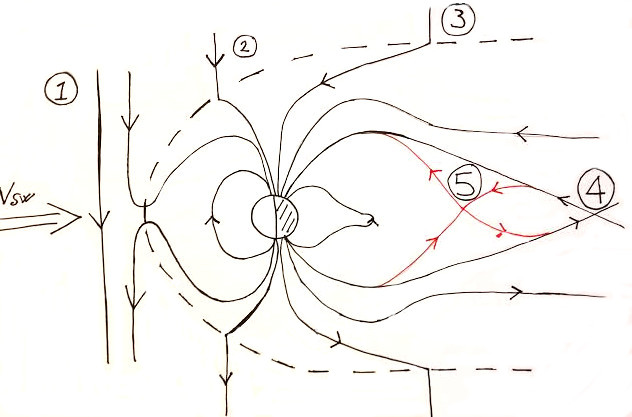
\includegraphics[scale=0.5]{solvind2.jpg}
\end{figure}

\subsection{Currents \label{_CHAP_THEO_currents}}

When we are dealing with the interaction of Earth's magnetic field with the IMF, it seems to be reasonable to investigate how the currents close to Earth behave.
The reason for this is due to the connection of magnetic fields and flowing currents. We know from Maxwell's equations that flowing electric currents cause a magnetic field. In particular,this relation is given by Ampere's law from Maxwell's equations. The important Maxwell equation is:
\begin{align}
\nabla \times \vec{B}= \mu_0 \cdot \vec{J} + \mu_0 \epsilon_0 \frac{\partial }{\partial t} \vec{E}
\end{align}
We can neglect the time dependence of the electric field in comparison with the $\vec{J}$-term and get ampere's law:
\begin{align}
\nabla \times \vec{B}= \mu_0 \cdot \vec{J}
\end{align}
Therefore, we can derive the current flow by looking at the magnetic field. In particular by looking at the curl of the magnetic field. (see AMPERE measurement)
In general, we can express the current flow in a given system with given magnetic field and electric field as follows:

\begin{align}
\vec{j}&= e n ( \vec{v}_i - \vec{v}_e ) = \sigma_p \vec{E}'_{\perp} + \sigma_H \frac{\vec{E}'_{\perp} \times \vec{B}}{B} + \sigma_{\parallel} \vec{E}_{\parallel}
\end{align}

Here, $\sigma_p$ is the Pedersen conductivity, $\sigma_H$ is the Hall conductivity and $\sigma_{\parallel}$ is a conductivity, which belongs to 
the electric field. We notice that the different currents caused by different conductivities flow in orthogonal directions with respect to each other. The orientation of $\vec{E}$ means parallel or orthogonal to the magnetic field. A discrete expression of the conductivities will not be needed in this report.

\iffalse 
\begin{align}
\vec{E}&= \vec{E}_{\perp} +\vec{E}_{\parallel}\\
\vec{E}'_{\perp}&=\vec{E}_{\perp}+ \vec{v}_n \times \vec{B}\\
\vec{E}'_{\perp}& \approx \vec{E}_{\perp}
\end{align}
\fi
\subsubsection{Earth's current system \label{_CHAP_THEO_currentsystem earth}}

The magnetic field of the terrestrial magnetosphere is produced by superposition of magnetic fields from a variety of sources.\cite{Buch2}[p.400]
Near Earth's surface, the biggest contribution comes from the currents within Earth's liquid core. However, electric currents like the solar dynamo, the equatorial electrojet, the convection electrojets and the substorm electrojets play also an important role. \cite{Buch2}[p.400]. 
We want to give a short overview about the current system of Earth. We want to limit us to currents, which can actually be measured by the instruments used in this report. The currents, which flow near the polar cap can be described as follows:
On the polar cap, we find Hall currents, Pedersen currents and Field-aligned currents. 
The characterisation of these currents is shown in \ref{_CHAP_THEO_currents}. When we want to describe the ionospheric currents, it is important to relate the gyro-frequency of electrons ($\omega_e$) and ions ($\omega_i$) to their collision frequency ($\gamma_e,\gamma_i$). The altitude profile of the collision-frequency of the two particles are not the same. This is due to different mass of the particles and therefore different particle-densities of the particles at given altitude. When electrons and ions gyrate much faster than they collide, both $\vec{E}\times \vec{B}$-drift and there is no total current. This is the case for altitudes above 120 km. For altitudes between 80 km and 120 km, ions collide more often than they gyrate. Therefore, ions move in the direction of $\vec{E}$. The electrons still gyrate faster than they collide. Therefore, electrons still $\vec{E}\times \vec{B}$-drift. In total, we can observe a current. Below 80 km altitude, electrons and ions collide more often than they gyrate. Both particles move along $\vec{E}$. There is no total current below 80 km altitude.
The layer from 80 km to 120 km is called the dynamo layer. 
Magnetic reconnection on day- and nightside enrols the so called twin cell convection. The twin cell convection belongs to a $\vec{E}\times \vec{B}$-movement. Since this drift is in general not charge dependent, there is no total current, when electrons and ions both $\vec{E}\times \vec{B}$-drift. As described above, there exists a layer, where electrons $\vec{E}\times \vec{B}$-drift and ions move in the direction of $\vec{E}$. In this layer, we can observe the so called electron hall-currents. The movement of the electron hall currents is twin cell shaped. (compare chapter \ref{_CHAP_THEO_twin cell convection}) This movement leads to an electric field, which can be described by $\vec{E}=-\vec{v}\times \vec{B}$. When only the ions move along $\vec{E}$, this leads to another current called the Pedersen current. Looking at the Pedersen-current-distribution, we can see that the Pedersen currents are not source free. However, it is necessary to close current systems. At the divergences of the Pedersen-currents, we promote currents. These currents are field aligned currents and close the Pedersen-currents. 
In the following, we shortly want to locate the different currents. 
The electron Hall currents flow at lower altitudes than the Pedersen currents. The flow of the Hall currents is also associated with the so called twin cell convection.
The ionospheric Pedersen currents are connected to the Field aligned currents (FAC). The FAC are on one side closed to the magnetopause current and on the other side closed by the ring current. These field aligned currents were discovered by a Norwegian scientist, Kristian Birkeland in 1908. All current systems must to be closed, which is also the case. The current flow on the polar cap can be seen in figure \ref{electric currents on the polar cap}.

\begin{figure}[h]
\centering
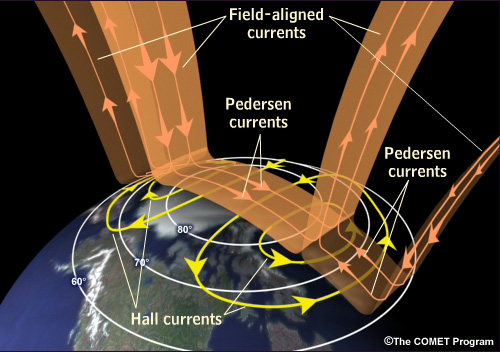
\includegraphics[width=0.5\textwidth]{polar_electric_currents.jpg}
\caption{electric currents on the polar cap\cite{Link1}}
\label{electric currents on the polar cap}
\end{figure}

\subsection{Twin cell convection \label{_CHAP_THEO_twin cell convection}}
If we look at the Dungey cycle ($B_z<0$), we can figure out the movement of the open/closed field lines at the polar caps, which gives us the movement of the particles at the polar cap. Let us first explain, what leads to the so called "Twin-cell"-convection. If we have southward IMF, the orientation of the IMF and Earth's magnetic field are opposite to each other and as we discussed in chapter \ref{_CHAP_THEO_Dungey cycle}, magnetic reconnection on the dayside of Earth can occur. 
The magnetic reconnection at the dayside adds open magnetic field lines to the polar cap. In other words, dayside reconnection adds magnetic flux to the polar cap. The deformation of the usually round open/closed-field boundary leads to a movement, which tries to "smooth out" the little bump in the boundary. 
Magnetic field lines naturally want to orientate in a straight line. 

If we now look at the nightside events, we know that magnetic reconnection occurs in the tail.(Dungey cycle) Reasons for this happening 
are for example that through dayside reconnection, magnetic flux is added to the tail, the magnetic pressure increases and leads in the end to magnetic reconnection in the tail. The magnetic reconnection to the tail closes open magnetic field lines. This means that the polar cap shrinks a bit on the nightside. 
In other words, magnetic flux is subtracted at the nightside of Earth from the polar cap. The subtraction leads to a little dint in the polar cap. 
The magnetic field lines tend to "smooth out" the little dint, which leads to a corresponding movement. 
In total, we expect now a movement, which is well known as the twin cell convection. The electric potential on the poles will give us the movement of the 
charged particles. The currents move along potential lines. The equipotential lines are therefore also the trajectories of the charged particles. 
The currents associated with that are called "Hall"-currents. The hall-currents can be found in an altitude of approximately 110 km. (electro-jets)


\section{Observations}

All in all, we use five different sources and data to draw an image of what is going on with the interaction of the IMF with Earth's magnetic field. We will just shorty list the used methods in this reports. A detailed description of each of the methods can be found in the separated chapters. 
First of all, we use a satellite called ACE (Advanced composition explorer) in order to get knowledge about the magnetic field of the IMF at Earth's position, which tells us whether dayside magnetic reconnection occurs or not . 
We also use The Ground-based magnetometer to get data from the magnetic field on Earth. Depressions in the magnetic field can be used to detect auroral substorms. 
Moreover, we want to look at data from SuperDARN in order to know the movement of charged particles in the ionosphere.
The data from AMPERE gives us a map of the Region 1 and Region 2 currents. Finally, the All-sky-Camera at Svalbard helps us to monitor and the intensity of the substorms.  

\subsection{ACE \label{0_CHAPTER_ACE}}
In this section, we want to discuss the data from the ACE. (Advanced Composition Explorer)
The ACE satellite orbits the Lagrangian point $L_1$.
\begin{figure}[h]
\centering
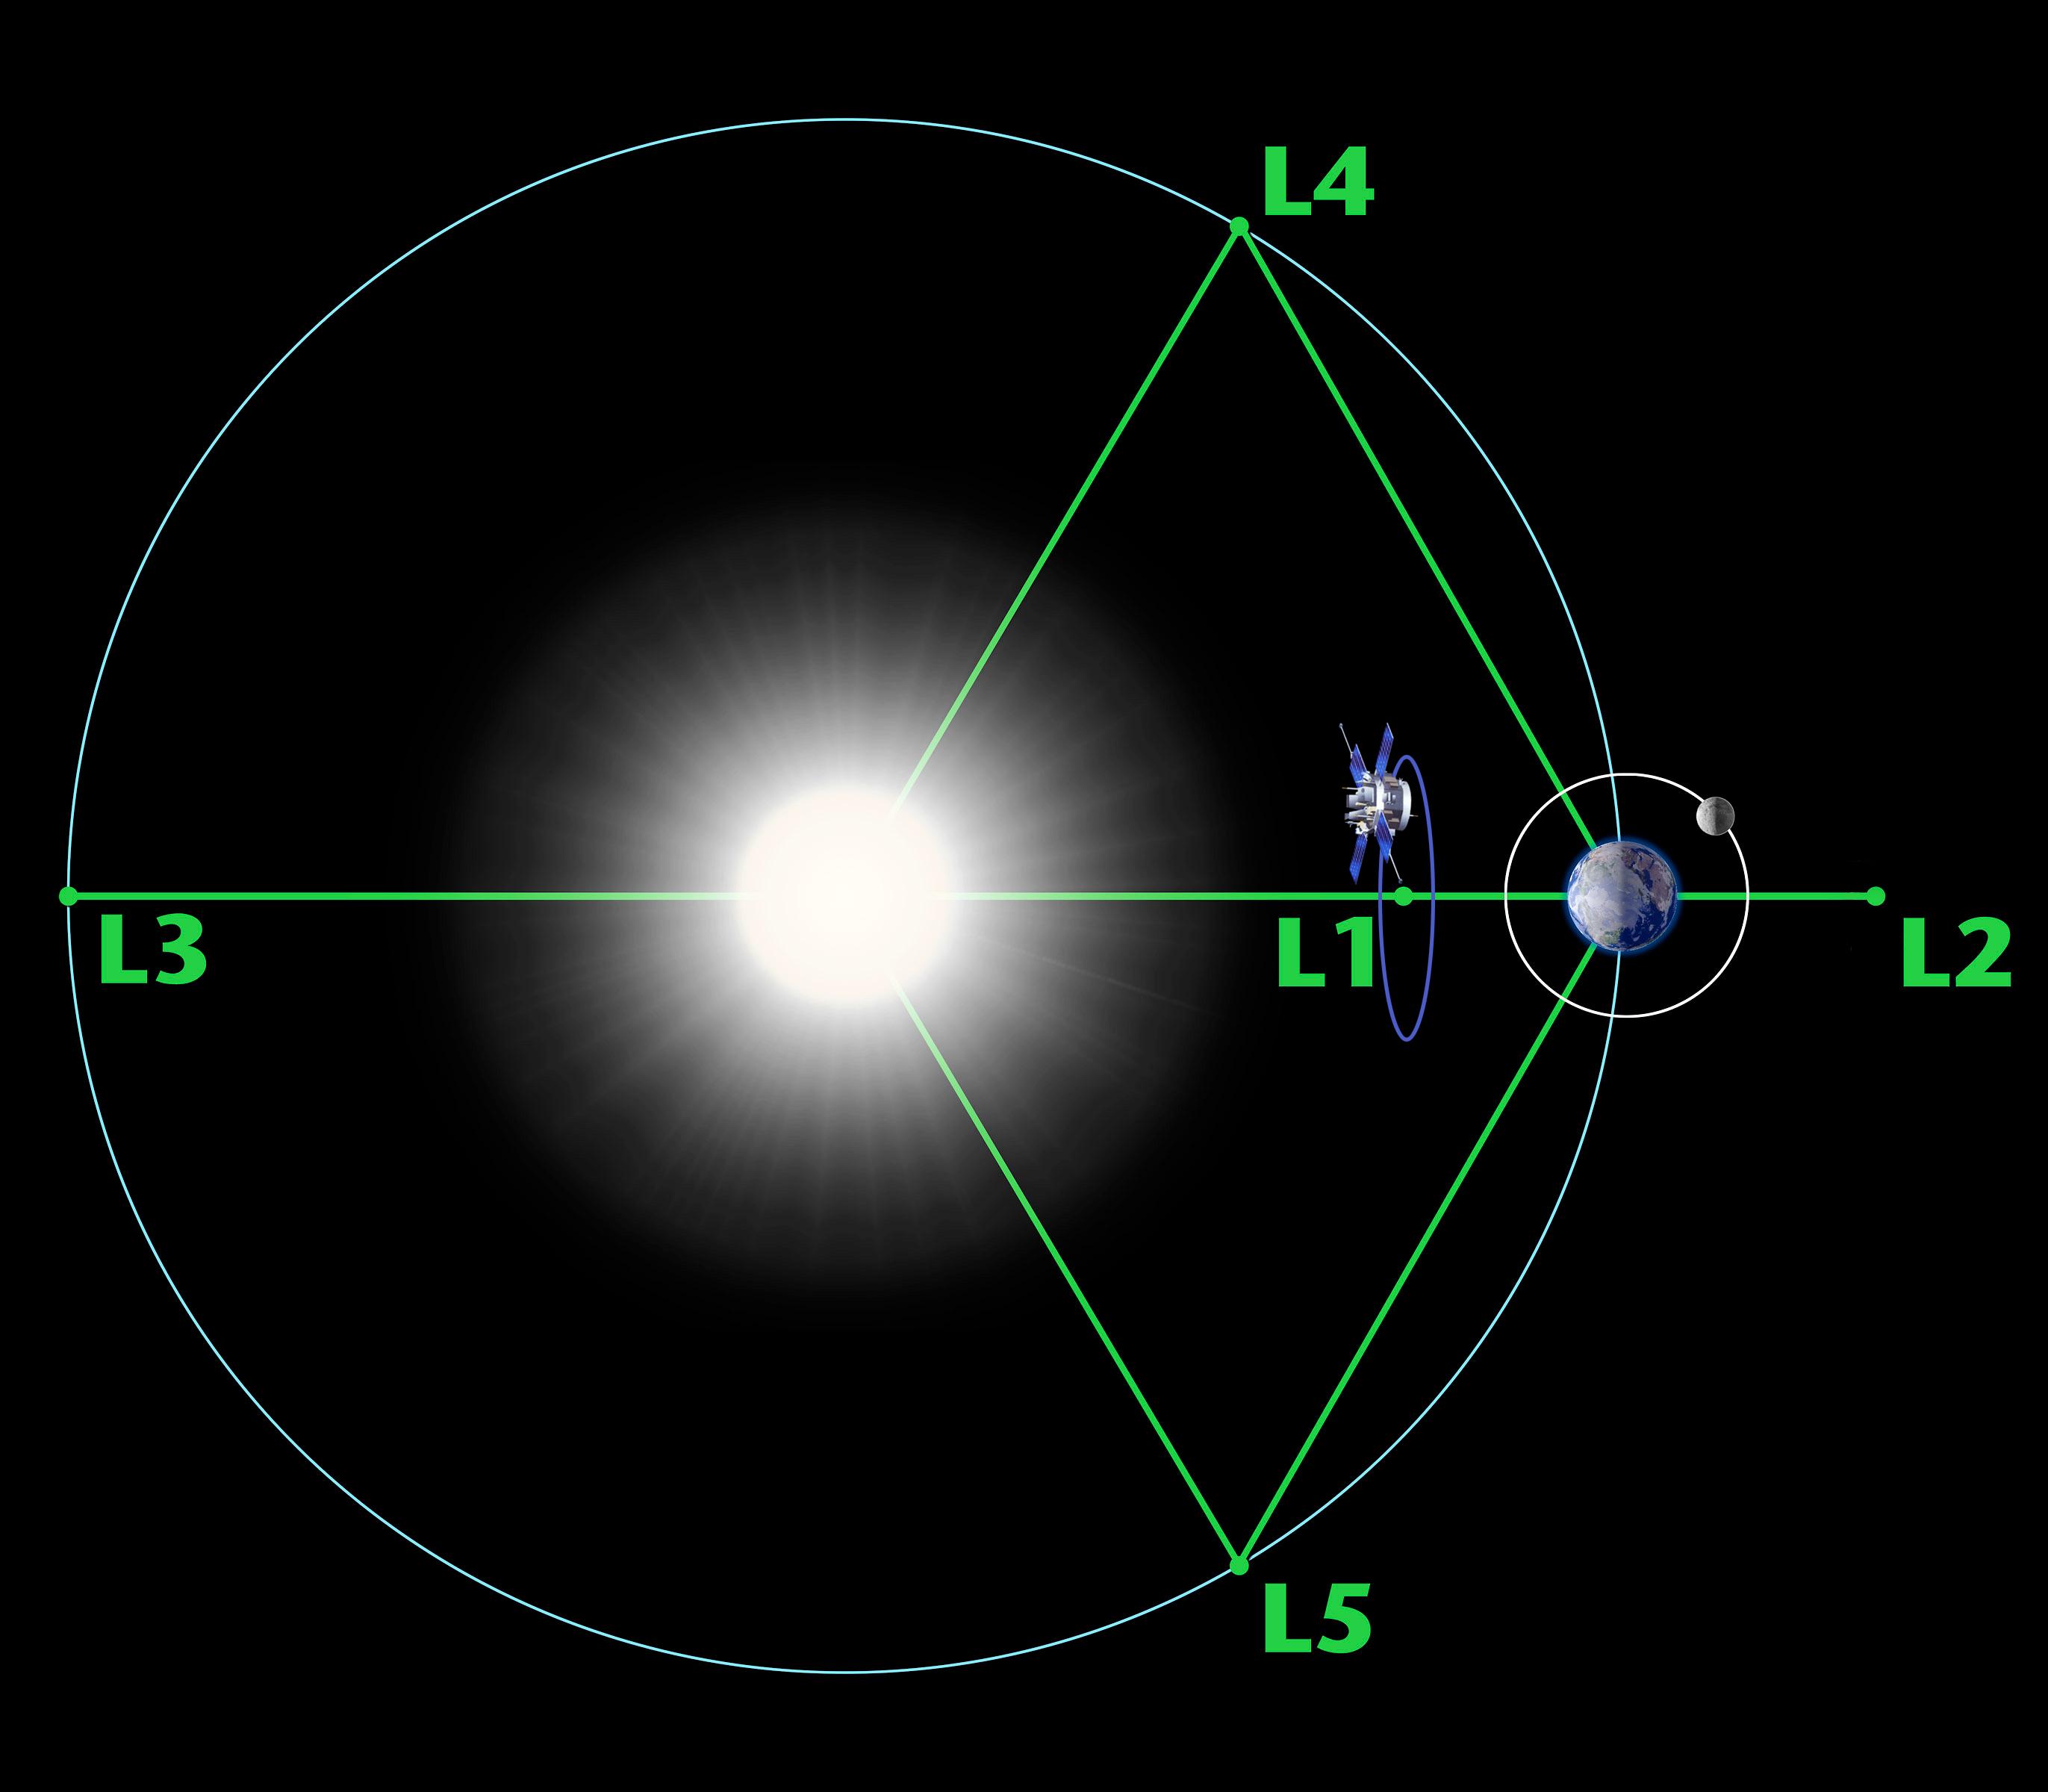
\includegraphics[scale=0.06]{ACEposition.jpg}
\caption{position of ACE \cite{Link2} }
\label{position of ACE}
\end{figure}

The Lagrange point L1 is located on the line between the Sun and the Earth, where the the gravitational forces are in equilibrium. (see figure \ref{position of ACE}) The solar wind particles move radially outwards from the Sun. Therefore, the data from ACE can be used to describe the IMF at Earth's position. Based on the solar wind bulk velocity and the distance from the satellite to the Earth, we make an approximation for when the solar wind reaches the Earth.

\begin{figure}[h]
\centering
\begin{subfigure}{0.45\textwidth}
\centering
	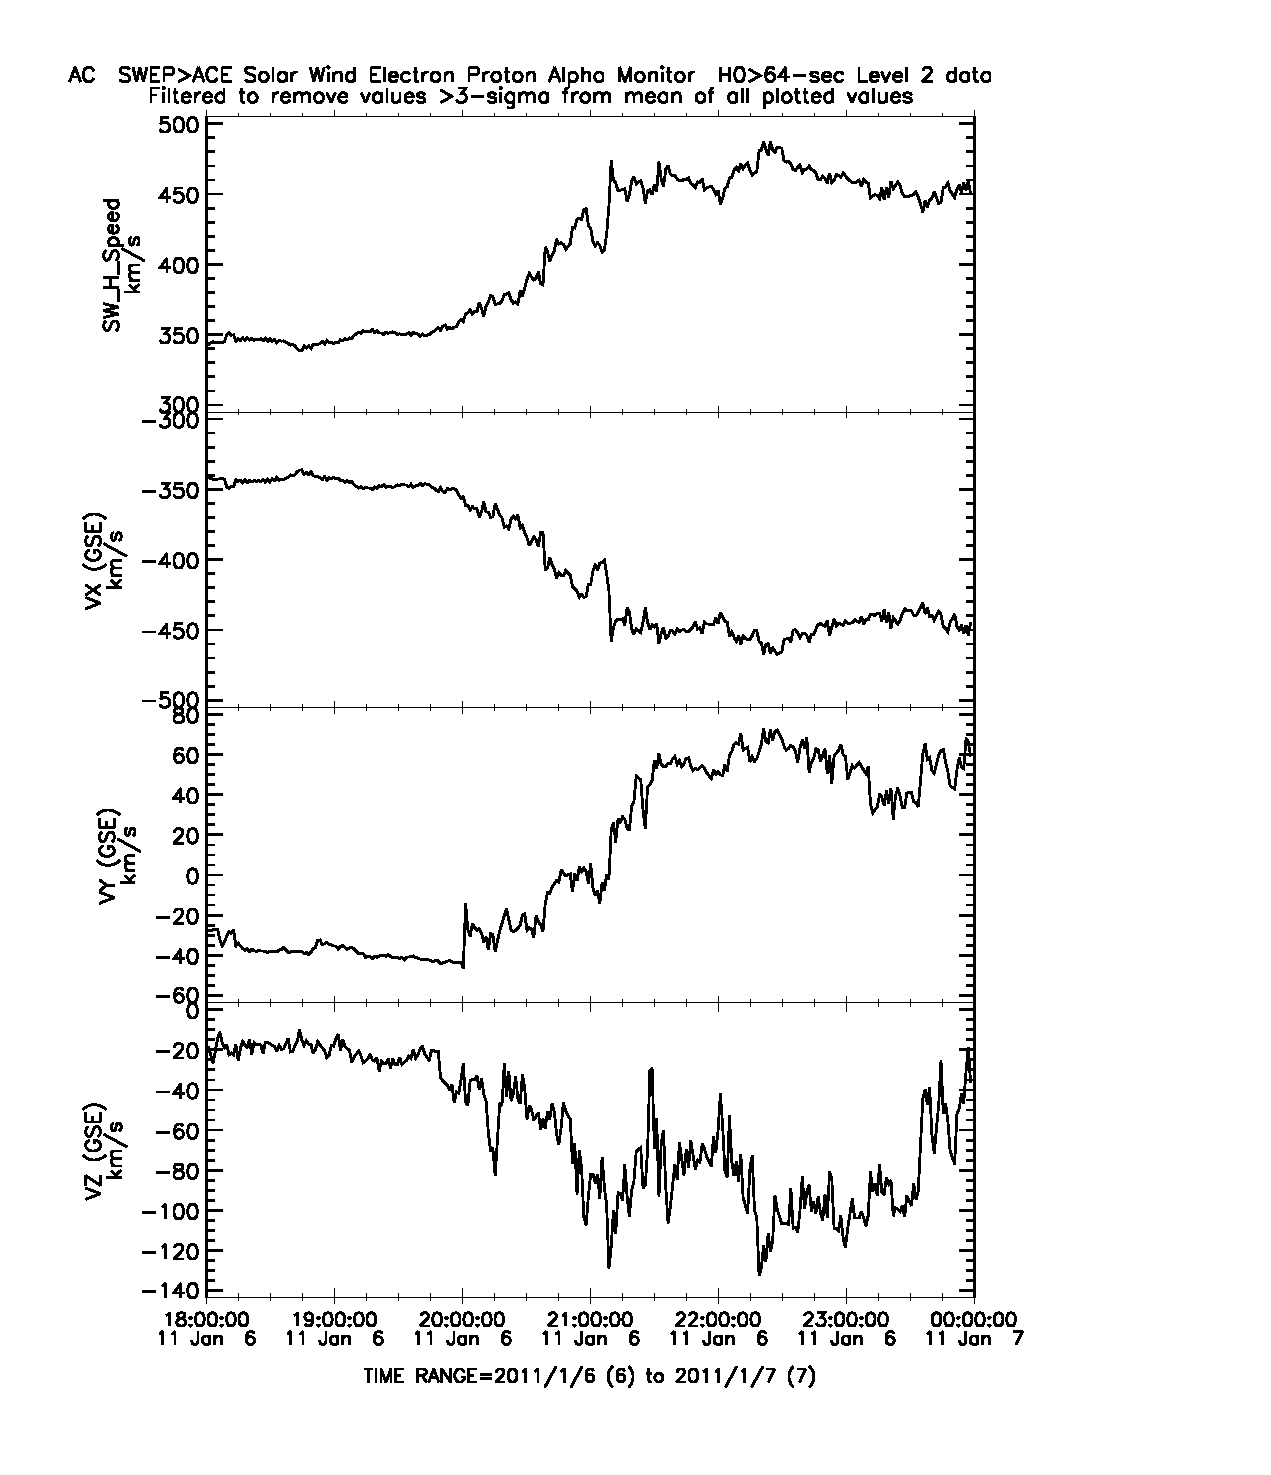
\includegraphics[width=\textwidth]{ACE_solarwindspeed.pdf}
	\caption{ Solarwind data\label{ACE Solarwindspeed}}
\end{subfigure}
\begin{subfigure}{0.45\textwidth}
\centering
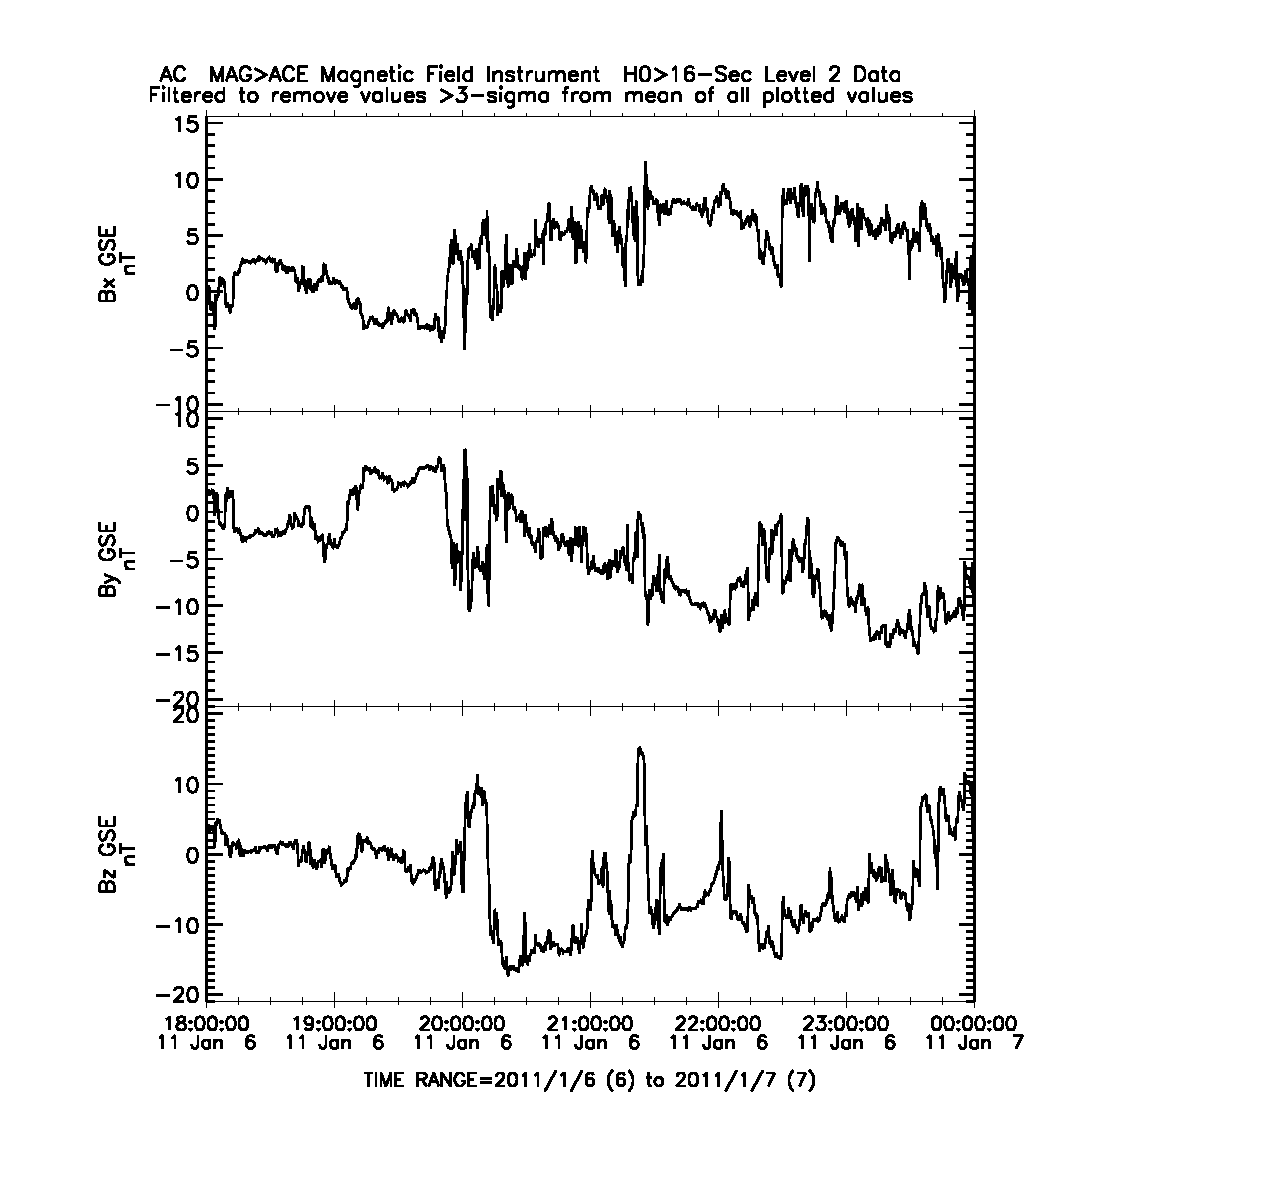
\includegraphics[width=\textwidth]{ACE_magneticfield.pdf}
\caption{magnetic field measured at the ACE}
\end{subfigure}
\caption{ACE data}
\end{figure}

\begin{figure}[h]
\centering
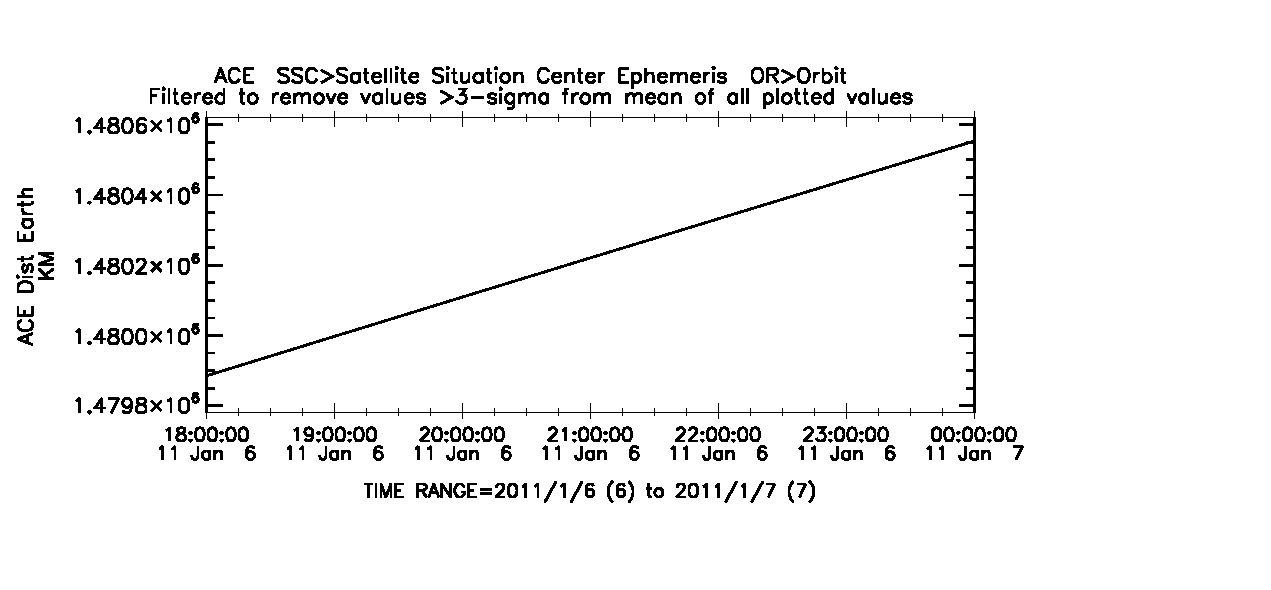
\includegraphics[width=0.5\textwidth]{ACE_distance.pdf}
\caption{ ACE distance from Earth \label{ACE distance}}
\end{figure}
We can therefore predict what the IMF looks like at Earth at a given time on Earth. This is important because we know from the chapter \ref{_CHAP_THEO_Dungey cycle}, that the $B_z$ tells us something about magnetic reconnection on the dayside. If $B_z>0$ (or northward IMF orientation), there is no magnetic reconnection on the dayside. There is no open magnetic flux added to the polar cap. However, if the $Bz$ component is negative (or southward orientation of IMF) magnetic reconnection on the dayside can occur and the Dungey cycle kicks in. It is therefore very important to get data from the $B_z$ component of the IMF. The other components of the IMF could be used at a later point to tell something about the specific shape of the twin-cell convection.(see paper\cite{paper2}) In figures \ref{ACE Solarwindspeed} and \ref{ACE distance}, we find data from the solarwindspeed and the ACE position. Both together will be used to determine the time delay of the IMF. For the data from ACE, we use the coordinate system GSE (Geocentric Solar Ecliptic). If we assume a average velocity of the solar wind (see \ref{ACE Solarwindspeed} $V_x$) of $400 \frac{m}{s}$ and a average distance of $1.4802 \cdot 10^{6} \mathrm{km}$ from ACE to Earth, we get a average time delay of 1 hour. (With values ranging from 55 minutes to 75 minutes.) From 18:00 UT to approximately 20:15 UT, the IMF at ACEs' position is slightly positive. We can see that the $B_z$-component of the IMF at the position of ACE turns negative at approximately 20:15 UT. The negative turn reaches Earth at approximately 21:25 UT.  
(to $B_z\approx-12 n T$ ) From there on, the IMF stays almost universally negative until 23:45 UT. At 21:20 UT, the $B_z$ component turned for a short time to relatively high positive values. 



\subsection{Ground-based magnetometer\label{0_CHAPTER_GROUNDBASEDMag}}

The Ground-based magnetometer we use is a collection of 32 station on the surface of Earth measuring the magnetic field. The collection is called 
IMAGE (International Monitor for Auroral Geomagnetic Effects). We have chosen a nightside event, which means that we have chosen a time when the All-sky-camera 
in Svalbard is on the nightside. If we have a look at our data, we should be aware of indications concerning auroral substorms. During a substorm, 
the westward electro-jets increase. The currents cause according to Ampere's rule a depression in the north-south component of the magnetic field on Earth. 
After the depression, the magnitude of the north-south component slowly increases to its original value.
Observing this depression is therefore a first hint of a substorm. Let us now have a closer look at the data. 

\begin{figure}[h]
\centering
\begin{subfigure}{0.3\textwidth}
\centering
	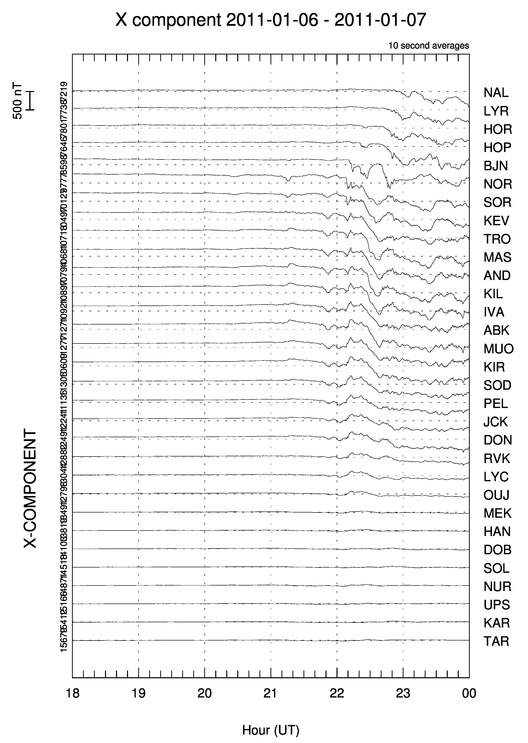
\includegraphics[width=\textwidth]{X_gram.jpg}
	\caption{ Groundbasedmagnetometer x-direction \label{GBM_X}}
\end{subfigure}
\begin{subfigure}{0.3\textwidth}
\centering
	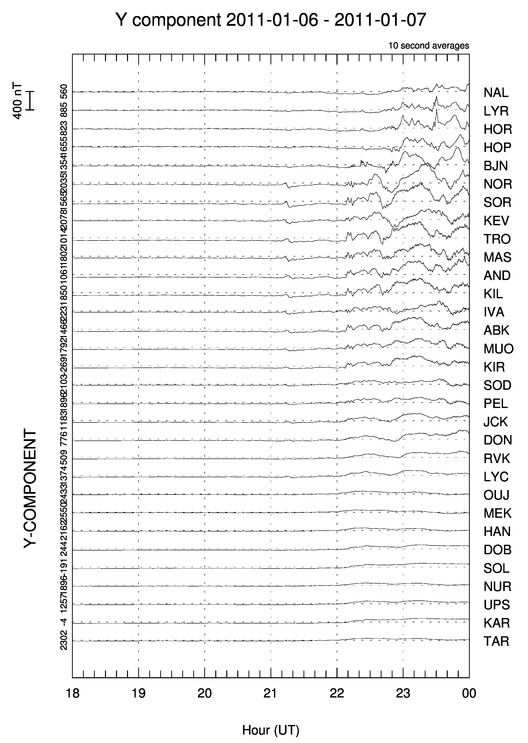
\includegraphics[width=\textwidth]{Y_gram.jpg}
	\caption{ Groundbasedmagnetometer y-direction \label{GBM_Y}}
\end{subfigure}
\begin{subfigure}{0.3\textwidth}
\centering
	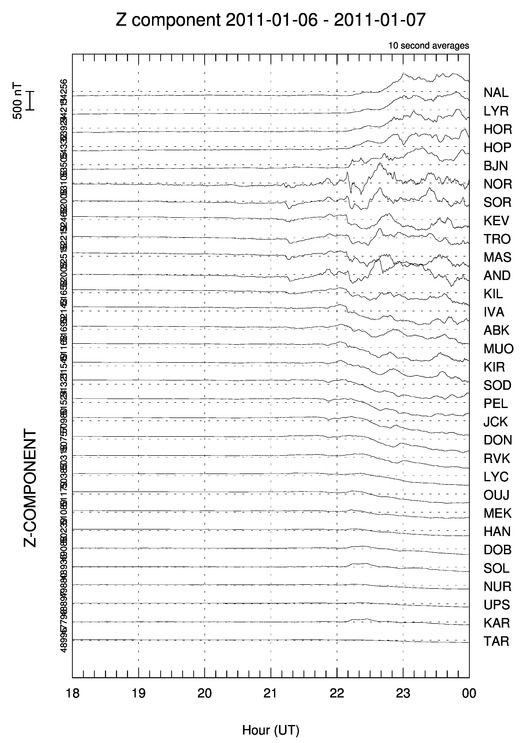
\includegraphics[width=\textwidth]{Z_gram.jpg}
	\caption{  Groundbasedmagnetometer z-direction\label{GBM_Z}}
\end{subfigure}
\caption{Data from Groundbasedmagnetometer, different components }
\label{GBM_all in all}
\end{figure}

In figure \ref{GBM_all in all}, you can see data from IMAGE. The figures \ref{GBM_X}, \ref{GBM_Y} and \ref{GBM_Z} show different orthogonal components of the magnetic field. In figure \ref{GBM_X}, you can see the south- north component of the magnetic field, which is the important component for us. The vertical axis of the plots show the time and the different horizontal lines are the magnetic field components measured at different stations on Earth. On the right side, you can see abbreviations of the different stations. Note, that they are ordered concerning their latitude. If you want to know where the station is exactly located, please have a look at figure \ref{Groungbasedmagnetometers_maps}.\\
The first thing, which strikes the eye is that the magnetic field component is mostly constant from 18:00 UT until approximately 22:00 UT. At approximately 22:00 UT (depends on the latitude of the station), we can see fluctuation of the magnetic field component and then a sudden depression of the magnetic field component. The first minimum of the measured magnetic field can be seen between 22:30 and 23:00 UT.
This is a hint to a substorm.(see chapter \ref{discussion} ) We can also see a poleward moving of the depression especially for the 8 most northward stations (KEV to NAL). We can also see that the stations MEK to TAR don't measure a depression of the magnetic field. The stations KEV to OUJ measure the depression approximately at the same time. 


\subsection{SuperDARN \label{0_CHAPTER_SUPERDARN}}
SuperDARN stands for  Super Dual Auroral Radar Network and this network consists of more than 30 low-power HF radars that look into Earth's upper atmosphere. 
(from mid-latitudes to polar regions) The radars can among other things be used to measure the motion of charged particles in the ionosphere via the Doppler shift effect. 
(scattering of radiation) The motion of the plasma is interesting for us because we know what we expect from the plasma movement and would like to compare experimental data 
with theory. In the ionosphere at approximately 110 km altitude, we expect to see the twin cell convection if the orientation of the IMF is southward. The twin cell convection is therefore related to the Dungey cycle. 
How can we visualize the motion of the hall currents? Unfortunately, we do not have a complete data coverage all over the polar cap. Therefore, it seems to be useful 
to search for another way to visualize the motion of the plasma. The velocity of the hall currents is: $\vec{v}=\frac{\vec{E}\times \vec{B}}{B^2}$ and the formula for 
the electric potential ($\phi$) is: $\vec{E}=-\vec{\nabla} \phi$. It now tuns out that lines of equal potential are perpendicular to the electric field, which is also the case 
for the hall currents. It can be shown that indeed the electric potential can describe the motion of the hall currents, the currents move along equipotential lines. 
The data of the Radars (motion of plasma) is used to make an expansion in spherical harmonics for the electric potential. Into this expansion is also baked in that currents have to be closed, which leads to closed equipotential lines. We should be careful with interpreting the data due to a lack of coverage and properties of the expansion itself . The plotting of the potential can then be used to describe the plasma flow. 

\begin{figure}
\centering
\begin{subfigure}{0.3\textwidth}
\centering
	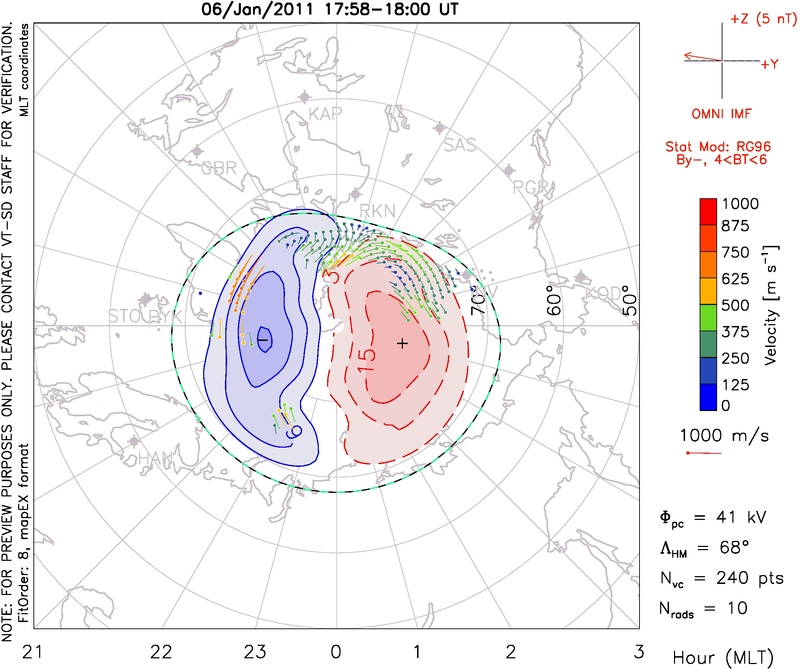
\includegraphics[width=\textwidth]{Superdarn1.jpg}
	\caption{ Superdarn at 18:00 UT \label{Super_18}}
\end{subfigure}
\begin{subfigure}{0.3\textwidth}
\centering
	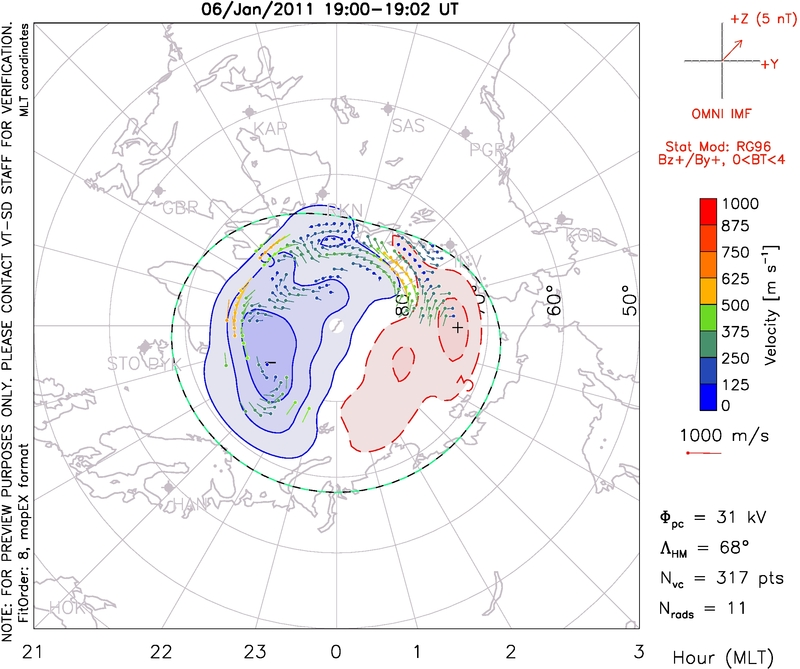
\includegraphics[width=\textwidth]{Superdarn2.jpg}
	\caption{ Superdarn at 19:00 UT \label{Super_19}}
\end{subfigure}
\begin{subfigure}{0.3\textwidth}
\centering
	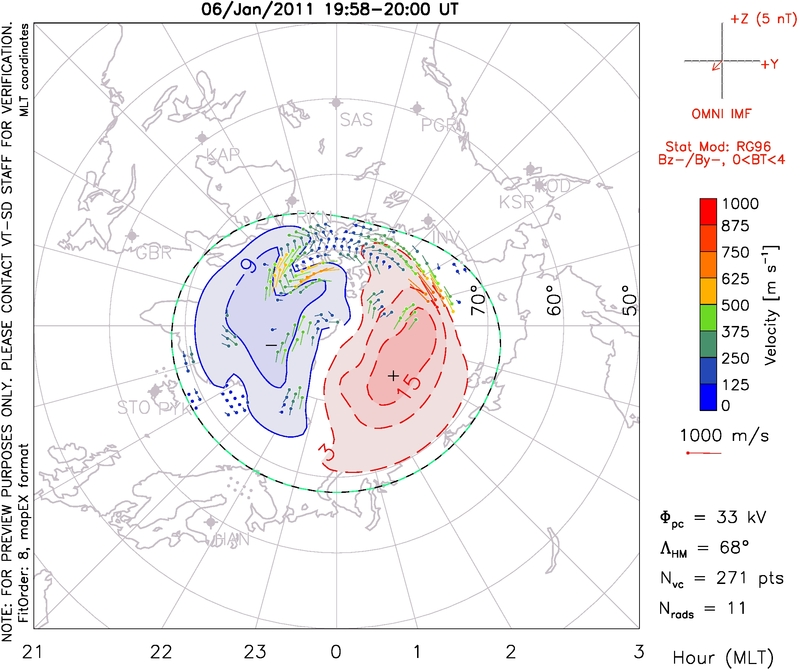
\includegraphics[width=\textwidth]{Superdarn3.jpg}
	\caption{ Superdarn at 20:00 UT \label{Super_20}}
\end{subfigure}
\begin{subfigure}{0.3\textwidth}
\centering
	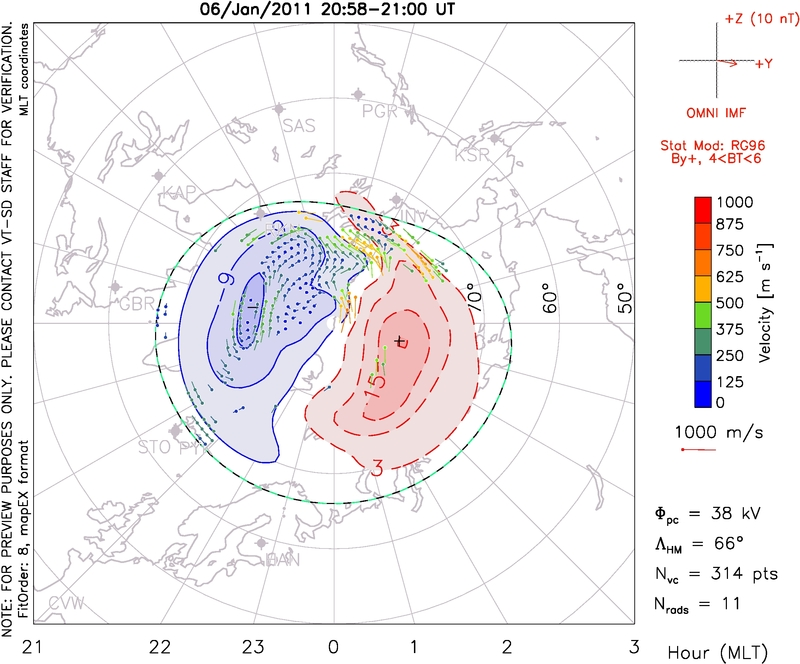
\includegraphics[width=\textwidth]{Superdarn4.jpg}
	\caption{ Superdarn at 21:00 UT \label{Super_21}}
\end{subfigure}
\begin{subfigure}{0.3\textwidth}
\centering
	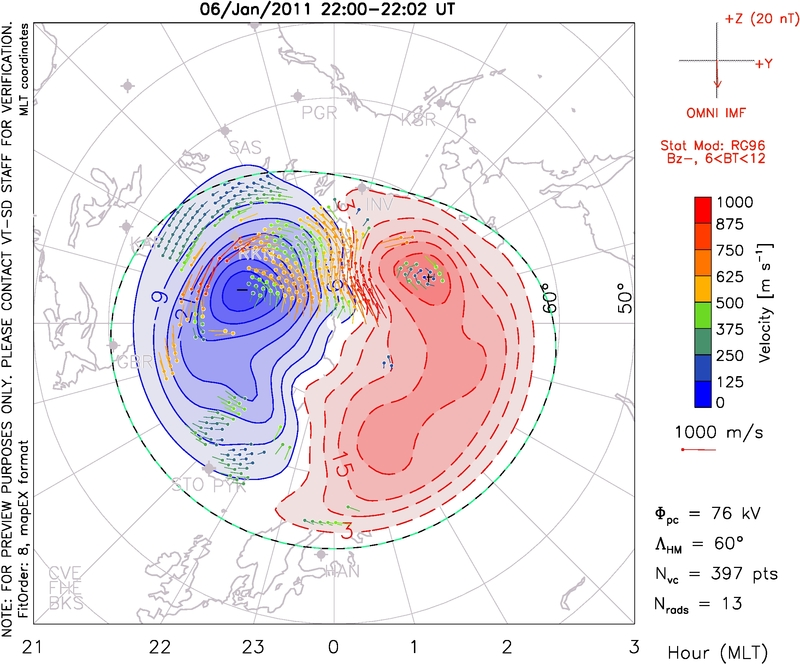
\includegraphics[width=\textwidth]{Superdarn5.jpg}
	\caption{ Superdarn at 22:00 UT \label{Super_22}}
\end{subfigure}
\begin{subfigure}{0.3\textwidth}
\centering
	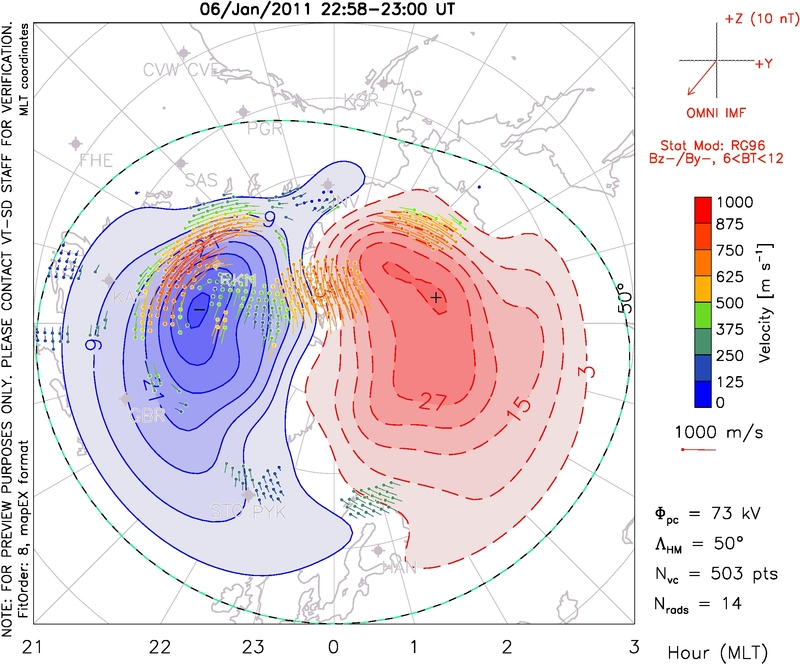
\includegraphics[width=\textwidth]{Superdarn6.jpg}
	\caption{ Superdarn at 23:00 UT \label{Super_23}}
\end{subfigure}
\begin{subfigure}{0.3\textwidth}
\centering
	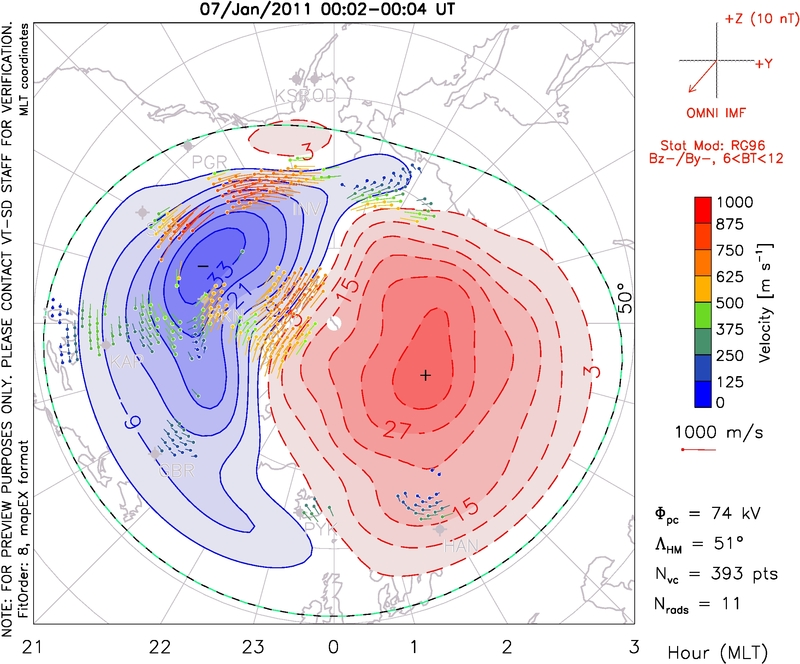
\includegraphics[width=\textwidth]{Superdarn7.jpg}
	\caption{ Superdarn at 00:00 UT, next day \label{Super_00}}
\end{subfigure}
\begin{subfigure}{0.3\textwidth}
\centering
	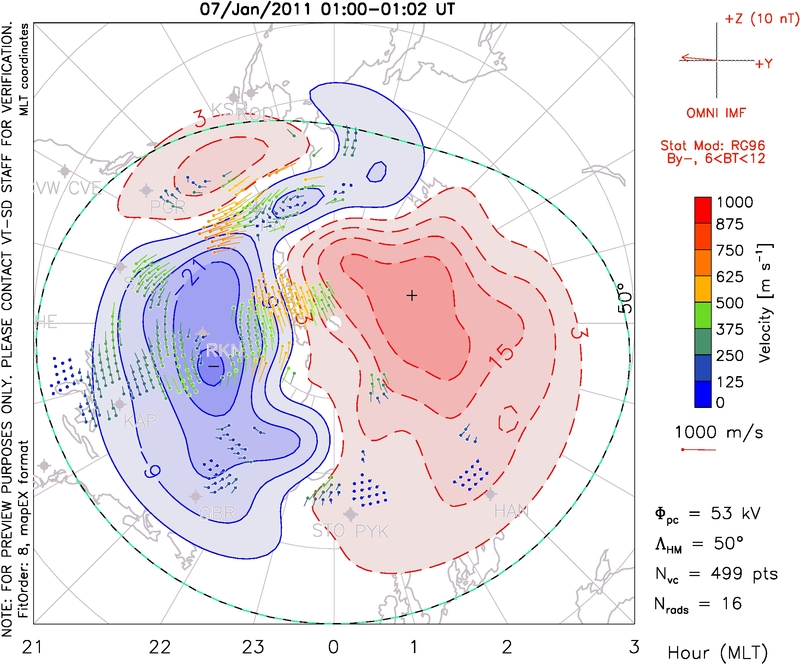
\includegraphics[width=\textwidth]{Superdarn8.jpg}
	\caption{ Superdarn at 01:00 UT \label{Super_01}}
\end{subfigure}
\begin{subfigure}{0.3\textwidth}
\centering
	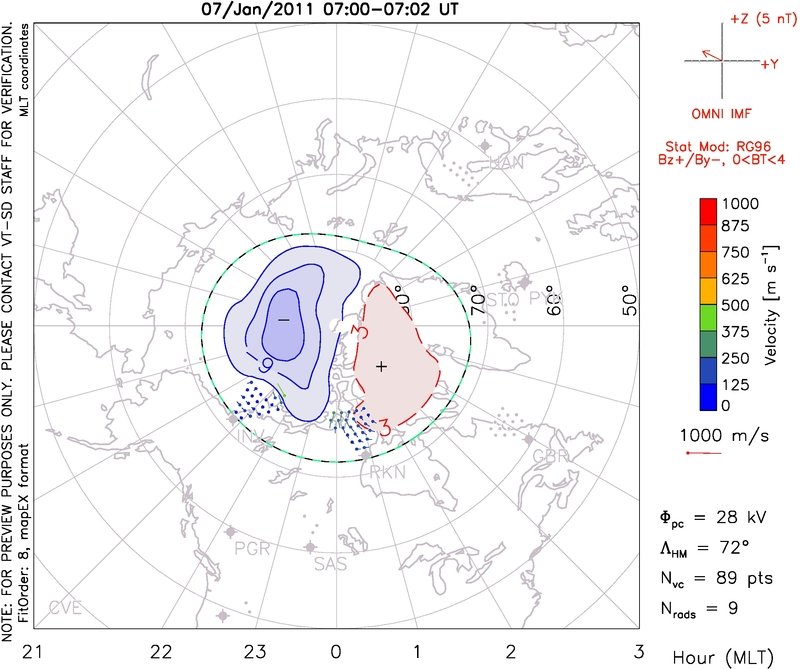
\includegraphics[width=\textwidth]{Superdarn14.jpg}
	\caption{ Superdarn at 07:00 UT \label{Super_07}}
\end{subfigure}
\caption{data from Superdarn for different times}
\label{Super_overview}
\end{figure}

The plot of the electric field on the polar cap is shown in figure \ref{Super_overview} for different times. For all figures you can qualitatively see two regions. One region with a positive electric potential in the dawn-region and one region with a negative electric potential in the dusk-region. The orientation of there "cells" is qualitatively the same. (two cells are separated by a line, which goes from noon to midnight) (look at figure \ref{Super_overview}) 
The strength of the electric potential variates a lot with time. We can compare the strength by comparing the contour lines of the potential. 
"The total strength of convection is characterised by the polar-cap potential drop" \cite{Buch2}[p.302]. From 18:00 UT to 21:00 UT, we have approximately the same 
strength of the electric potential. At this time, we also have approximately the same magnetic open flux through the polar cap. $\phi_{pc}=31kV$ to $\phi_{pc}=41 k V $. 
The size of the polar cap stays the same in this time interval. We can also see that the area, where the electric potential is significantly different from 0 is fairly small and located at high latitudes. (above 70\textdegree $
\;$ north)(see figures \ref{Super_18} to \ref{Super_21})
At 22:00 UT, we can see a huge difference to the previous time step. The strength of the electric potential increases. The area of electric potential, which is significantly different from 0, is increased from about 66\textdegree $\;$ to about 60\textdegree $\;$ latitude. The open magnetic flux through the polar cap is now $\phi_{pc}=76 k V$. (see figure \ref{Super_22})
At 23:00 UT on the 6th of January 2011, The area expands even more and the potential reaches its maximum from all the shown time frames. (expanded almost to 50 \textdegree $\;$ 
latitude) The strength of the electric field stays approximately the same as well as the open magnetic flux through the polar cap. (see figure \ref{Super_23})
At 00:00 UT on the 7th of January 2011, the properties described at 23:00 UT stay the same. However, we see on the top of figure \ref{Super_00} a small but 
separated blob of positive potential, which we couldn't observe at 23:00 UT. There are no data points in the blob itself, which makes it un-probable that this is caused by real data. 
At 01:00 UT, we observe a weaker electric field than in the previous time step. We also observe some perturbations compared to the  "two-cell-observation" from the 
previous steps. These perturbations are probably not only caused by the expansion because we have data supporting the positive potential at noon. 

\newpage
\subsection{AMPERE \label{0_CHAPTER_AMPERE}}
AMPERE (Active Magnetosphere and Planetary Electrodynamics Response Experiment) is a Earth observing system, which can be used to measure near-realtime magnetic field by 66 commercial satellites. The data from the magnetic field collected by AMPERE can be used to improve our understanding of space weather. In our project, we want to use AMPERE to determine the Birkeland currents. The Birkeland currents are field aligned currents. As described in the theory part, flowing electric currents 
cause a curl of the magnetic field. If there are such FAC, we should also see a curl in the magnetic field measured by the satellites.
We don't want to have a look at the explicit magnetic field data, but directly at the simulated current flow based on the measured magnetic field of AMPERE. We expect to 
see two current regions. Region 1 currents flow in positive z-direction, while region 2 currents flow in the opposite, negative z-direction. The configuration 
of the electric fields set up by the movement of magnetic flux tubes across the polar cap is such that we expect region 1 \& 2 currents to lie inside each other like concentric circles. Furthermore we also expect that on the dayside the region one current is on the higher latitude while the region 2 currents are on the lower. Vice versa for the nightside. We are interested to see how these currents change with respect to time.  

\begin{figure}[h]
\centering
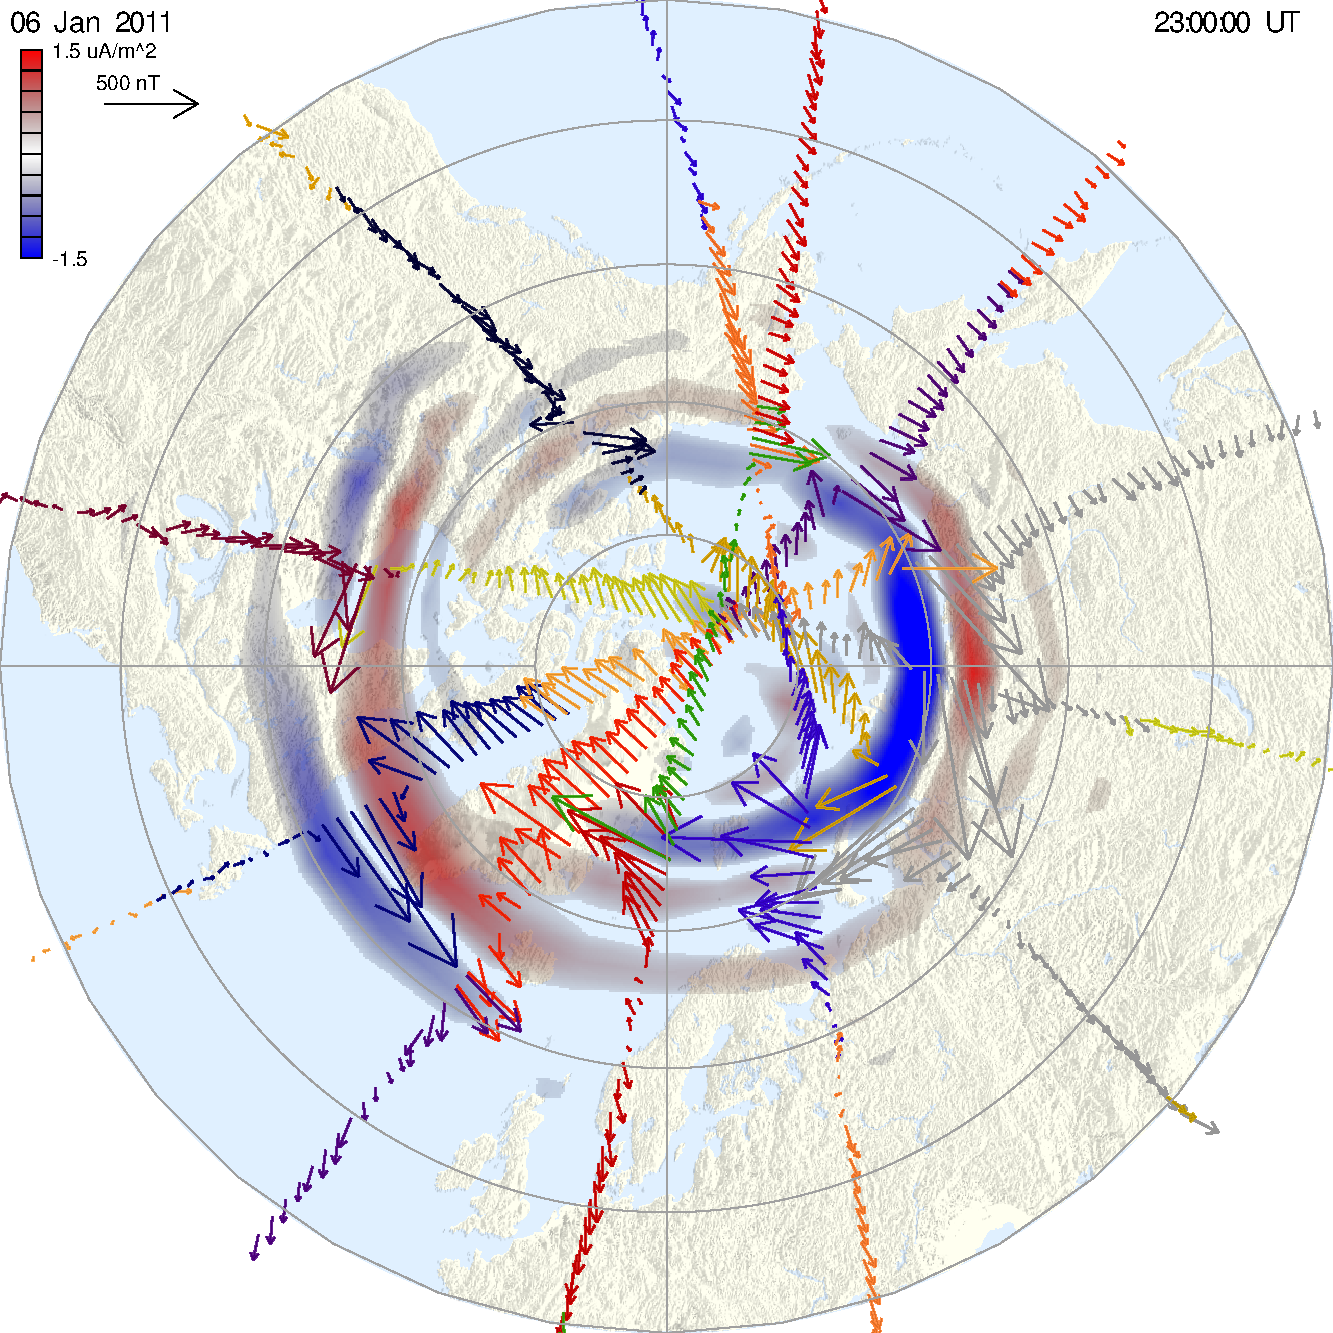
\includegraphics[scale=0.3]{summary_better_exp.pdf}
\caption{This figure shows the measured magnetic field vectors by the satellites at 23:00 UT of the 6th January and the field align currents in blue and red}
\label{AMPERE_explonation}
\end{figure}
In figure \ref{AMPERE_explonation}, we can see the measured magnetic field by the satellites visualized through little arrows. We convince ourselves that a curl in the magnetic field can be related to a area with blue or red colour, which belong to field aligned currents. Red colour means that the field aligned currents flow away from the surface of Earth and blue towards Earth. 
With this pre-knowledge, we can now have a closer look at the data. From 18:00 UT (see figure \ref{amp18}) until 20:00 UT(see figure \ref{amp20}), we don't see significant currents. At 21:00 UT (see figure \ref{amp21}), we see a small increase of the currents indicated by a bit more intensive red and blue colour. However, it is hard to derive a structure of the current-flow. At 22:00 UT (see figure \ref{amp22}), the current flow is a bit more intense than one hour before. We can now see four different areas. An inner circle consisting of a current coming down from space to Earth on the right half on the circle and of currents flowing into space the left part of the circle. The outer circle consists of a current coming down from space to Earth on the left half on the circle and of currents flowing into space on the right part of the circle. This basic structure can also be seen at 23:00 UT and at 00:00 UT.(see figure \ref{amp23} and \ref{amp00}) 
The currents reach their maximum at approximately 23:00 UT. From there on, the currents decrease. At 02:00 UT (see figure \ref{amp02}), we can say that there aren't any significant currents any more. 

\begin{figure}[h]
\centering
\begin{subfigure}{0.3\textwidth}
\centering
	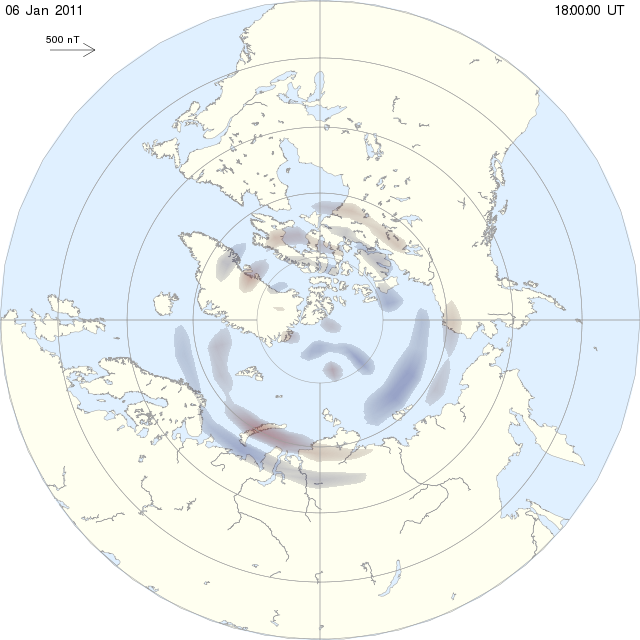
\includegraphics[width=\textwidth]{ampere0.png}
	\caption{ 18:00 UT\label{amp18}}
\end{subfigure}
\begin{subfigure}{0.3\textwidth}
\centering
	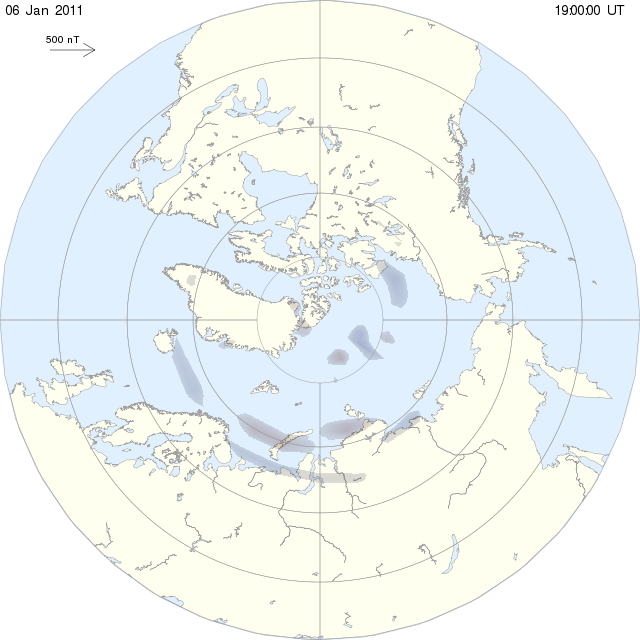
\includegraphics[width=\textwidth]{ampere1.png}
	\caption{19:00 UT \label{amp19}}
\end{subfigure}
\begin{subfigure}{0.3\textwidth}
\centering
	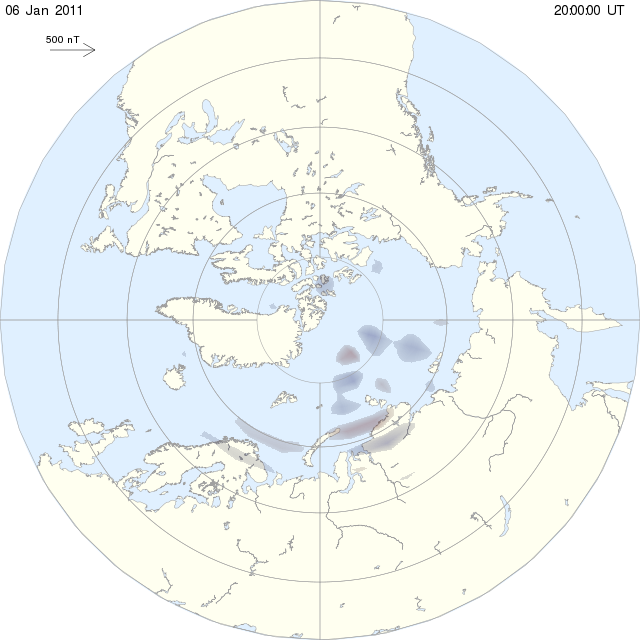
\includegraphics[width=\textwidth]{ampere2.png}
	\caption{ 20:00 UT \label{amp20}}
\end{subfigure}
\begin{subfigure}{0.3\textwidth}
\centering
	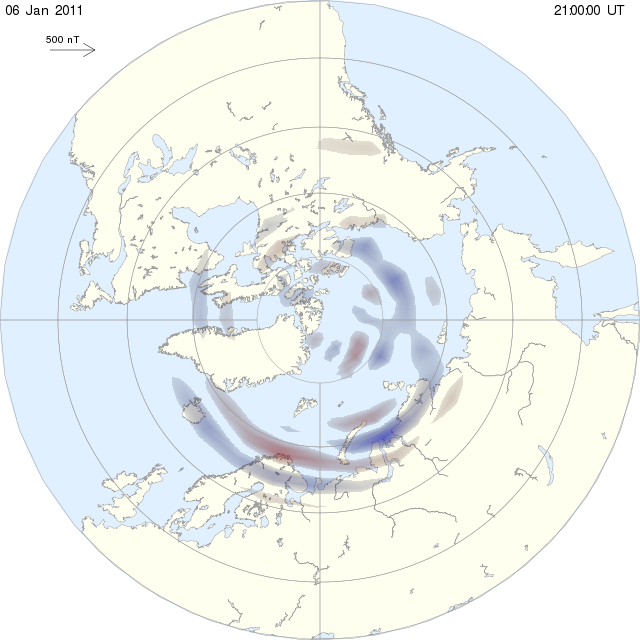
\includegraphics[width=\textwidth]{ampere3.png}
	\caption{ 21:00 UT \label{amp21}}
\end{subfigure}
\begin{subfigure}{0.3\textwidth}
\centering
	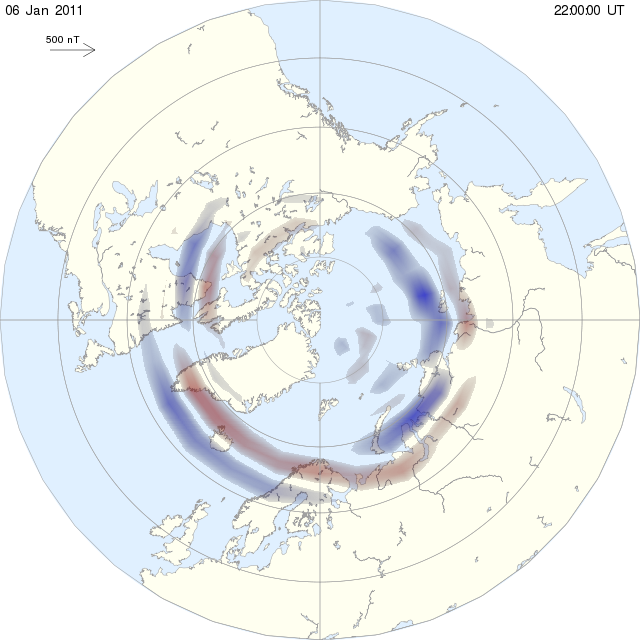
\includegraphics[width=\textwidth]{ampere4.png}
	\caption{ 22:00 UT \label{amp22}}
\end{subfigure}
\begin{subfigure}{0.3\textwidth}
\centering
	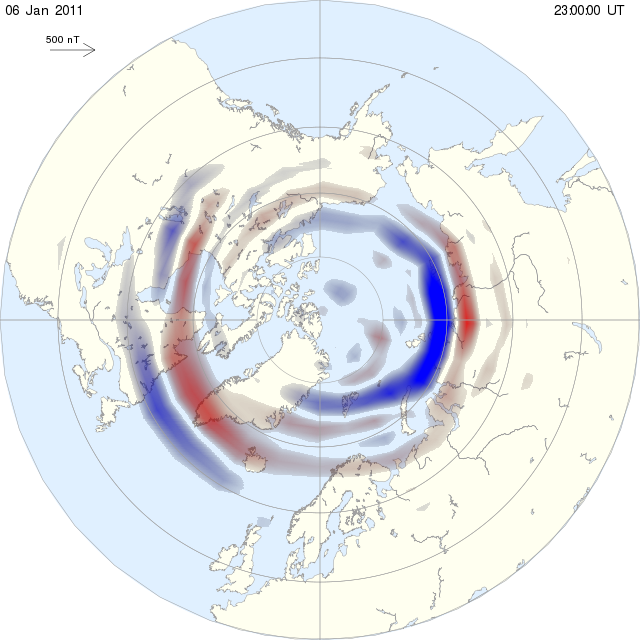
\includegraphics[width=\textwidth]{ampere5.png}
	\caption{ 23:00 UT \label{amp23}}
\end{subfigure}
\begin{subfigure}{0.3\textwidth}
\centering
	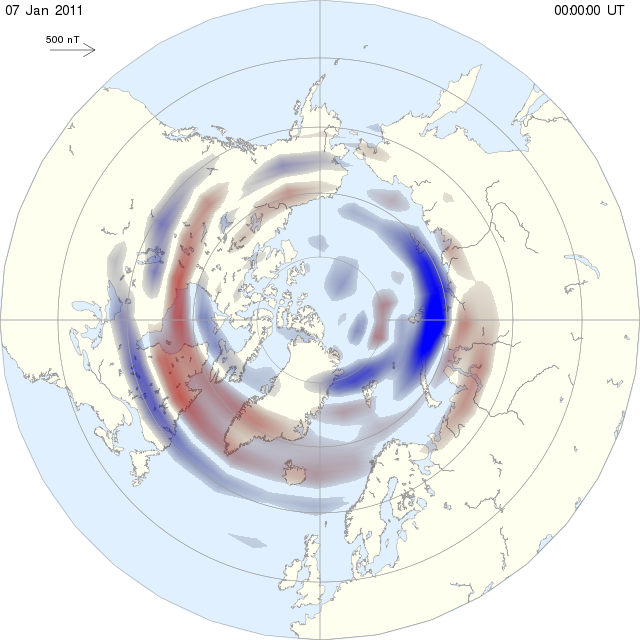
\includegraphics[width=\textwidth]{ampere6.png}
	\caption{ 00:00 UT (next day) \label{amp00}}
\end{subfigure}
\begin{subfigure}{0.3\textwidth}
\centering
	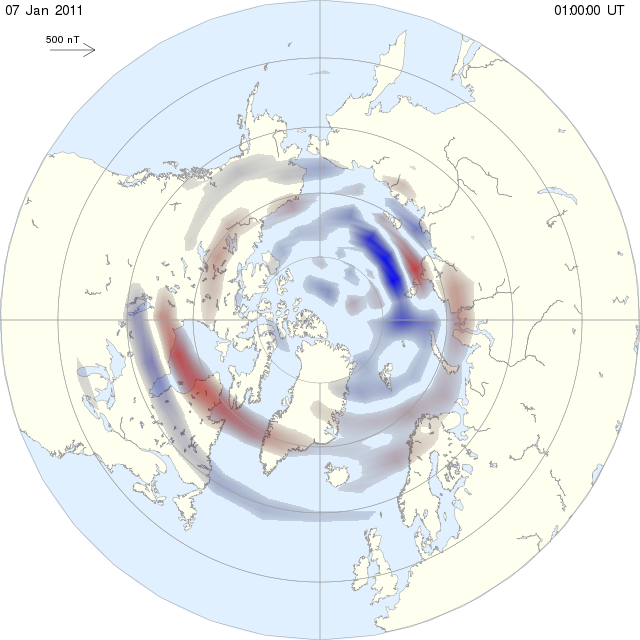
\includegraphics[width=\textwidth]{ampere7.png}
	\caption{ 01:00 UT \label{amp01}}
\end{subfigure}
\begin{subfigure}{0.3\textwidth}
\centering
	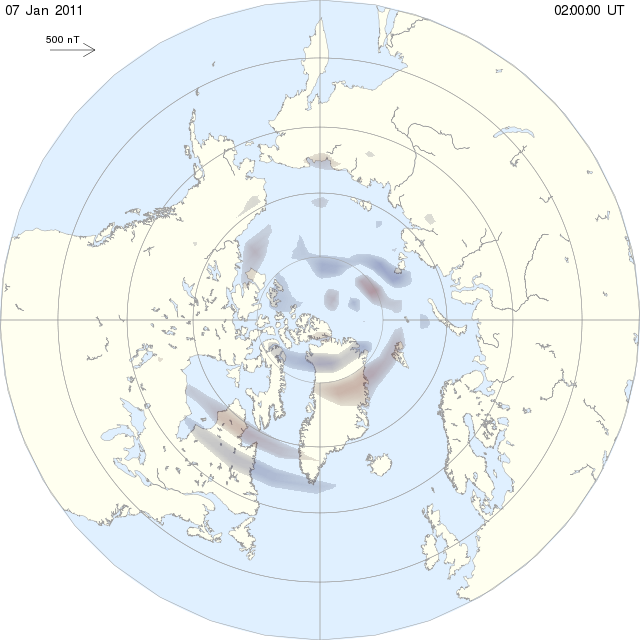
\includegraphics[width=\textwidth]{ampere8.png}
	\caption{ 02:00 UT \label{amp02}}
\end{subfigure}
\caption{Data from AMPERE at different times}
\end{figure}
\newpage
\subsection{Svalbard All-Sky Imager \label{0_CHAPTER_SVALBARDIM}}

The Svalbard All-Sky Imager measures the intensity of two different wavelength all over the sky. Every pixel represents a small part of the sky. We look at two different 
wavelength($\lambda_1=630 nm, \lambda_2= 557.7 nm$). The reason for this is that we want to have a look at the most important constituents of the northern lights. 
Aurora is caused by electrons and ions precipitating in the upper atmosphere. They collide with neutrals and thereby the electrons and ions can transfer energy to the neutrals while exciting the neutral atoms. When the neutrals relax from the excited state to the ground-state, they emit radiation. 
$\lambda_1$ belongs to the relaxation from the 1D orbital to the 3p orbital of atomic oxygen and $\lambda_2$ belongs to the relaxation from the 1s orbital to the 1D 
orbital. We have different images for each of these wavelengths. (compare reference \cite{Buch2}[p.469f] )
in order to visualize the time-development of the intensity of this light, it is convenient to use a so called keogram. A keogram takes a slice from the center of each 
image at each time  step and adds the different slices together in order to produce a timeline. Longitudinal movements are easily detected in keograms, however for 
the exact latitudinal movements one should check the full images. In the images, red areas represent relatively high intensity of the specific wavelength and black 
relatively low intensity. We should keep in mind that the intensities are rescaled for every picture in order to have a better visualization. 
The figure \ref{SBI_all_overview} shows a general overview of the whole day. (06.01.2011) Figure \ref{SBI_5_overview} shows the overview of the whole day for 
$\lambda_2$ and \ref{SBI_6_overview} shows the overview of the whole day for $\lambda_1$. The interval from 00 UT to 18:00 UT is not interesting for us. 
We can see that from 18:00 UT to approximately 22:00 UT, the intensity on both images are really low; whereas from 22:00 UT to 24:00 UT (7th January) 
we can see that we have high intensity over all longitudes represented by the red colour.

\begin{figure}[h]
\centering
\begin{subfigure}{0.45\textwidth}
\centering
	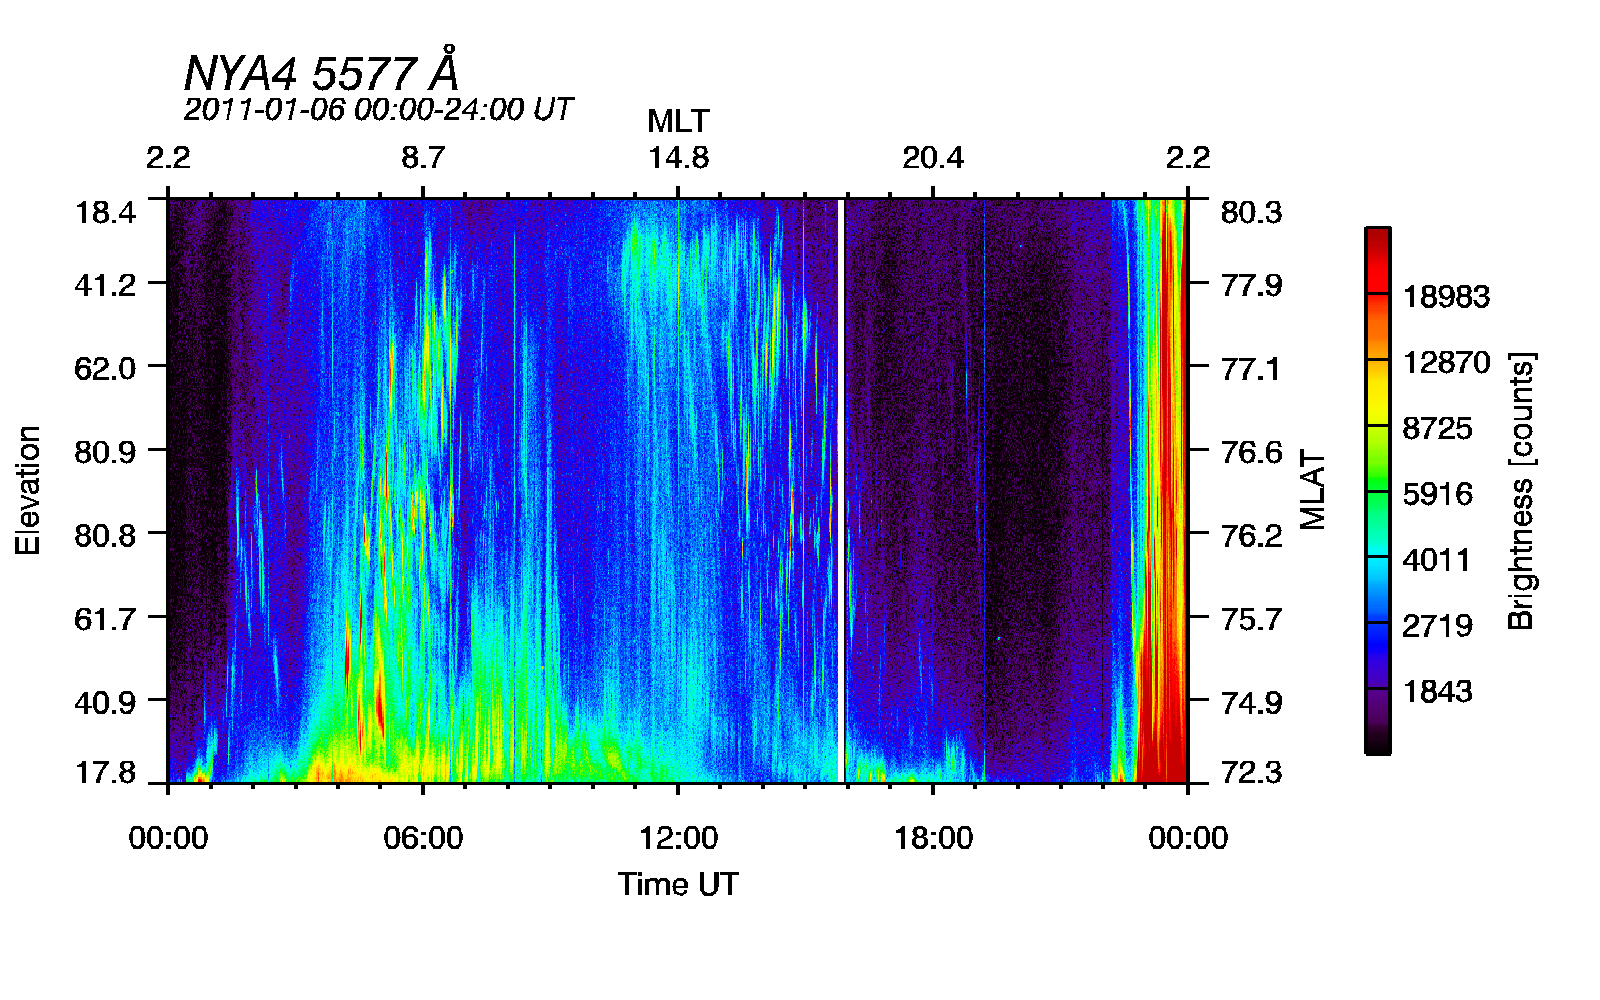
\includegraphics[width=\textwidth]{SvalbardImager5577A.png}
	\caption{ SvalbardImager for 5577 \AA{} \label{SBI_5_overview}}
\end{subfigure}
\begin{subfigure}{0.45\textwidth}
\centering
	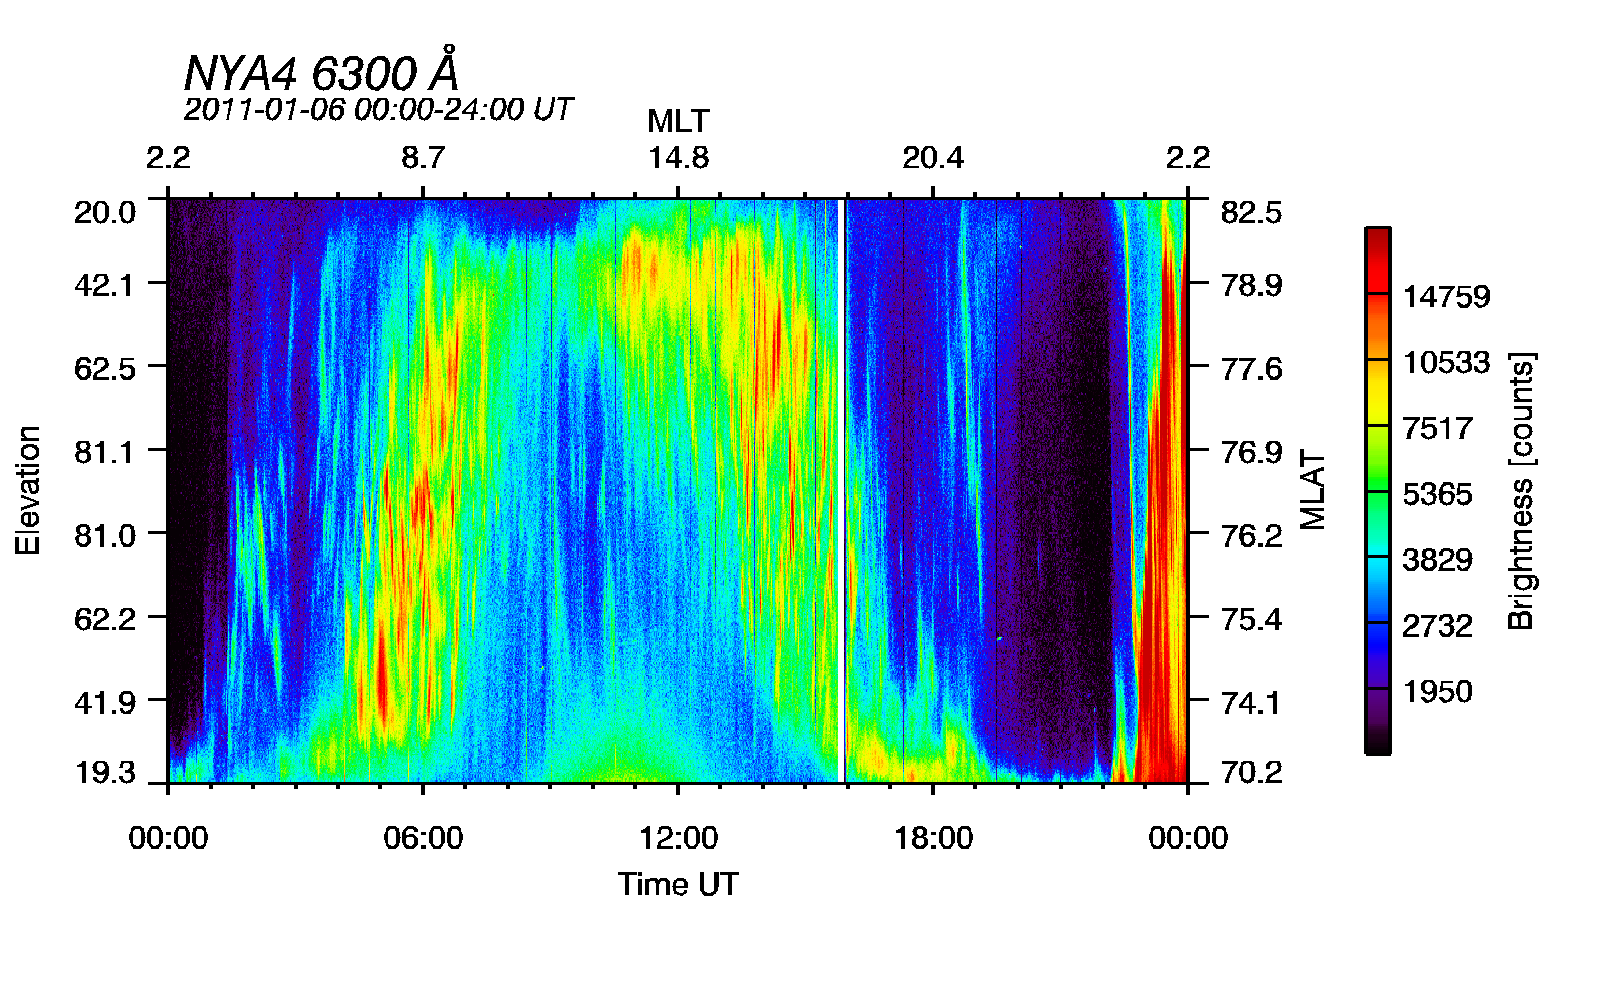
\includegraphics[width=\textwidth]{SvalbardImager6300A.png}
	\caption{ SvalbardImager for 6300 \AA{} \label{SBI_6_overview}}
\end{subfigure}
\caption{Overview over the Svalbard-Imagers}
\label{SBI_all_overview}
\end{figure}

In the figure \ref{SBI_5_overview}, we can see keograms from the whole period, with one hour intervals. In figure \ref{SBI_5_18} to \ref{SBI_5_21}, we don't see anything 
special. The red area at below $20$\textdegree is associated with the polar oval. At 22:30, we can see the first movement of an area of high intensity of light from north to 
south and at 22:45, we see a higher intensity of the light up to $76.5$\textdegree latitude. (see figure \ref{SBI_5_22})
At 23:00 UT, we can see a lot of areas with high light-intensity. The longest time interval of high light intensity all over the latitudes is at approximately 23:30 UT and lasts about 5-10 minutes. At 23:45 UT, the intensity is low and at 23:55, higher intensities are again measured at high latitudes. In figure (\ref{SBI_5_22}) we 
observe an interesting filament which could be a polar arc. We can see it moving from the very high latitudes at 22:30, then 15 minutes later it seem to merge with the auroral oval. At the same time as the polar arc merges with the auroral oval, over all intensity is on the rise, and shortly after we observe a very dynamic and active auroral display.  
\begin{figure}[h]
\centering
\begin{subfigure}{0.3\textwidth}
\centering
	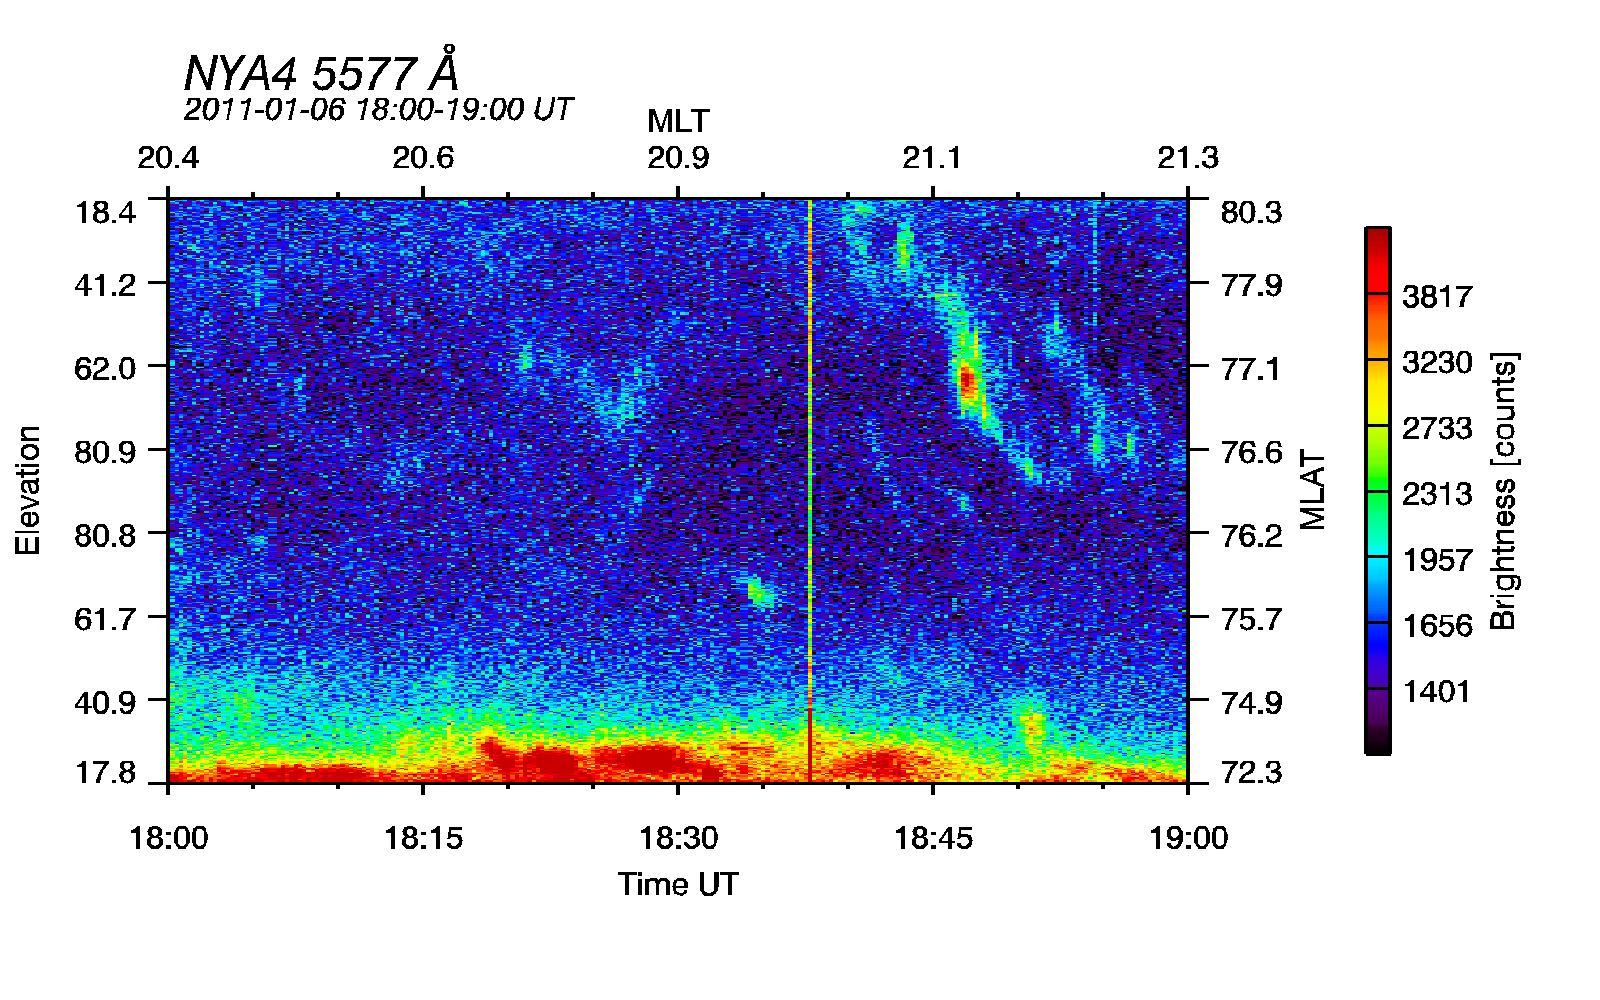
\includegraphics[width=\textwidth]{SvalbardImager5577A18.png}
	\caption{ SvalbardImager at 18:00 UT \label{SBI_5_18}}
\end{subfigure}
\begin{subfigure}{0.3\textwidth}
\centering
	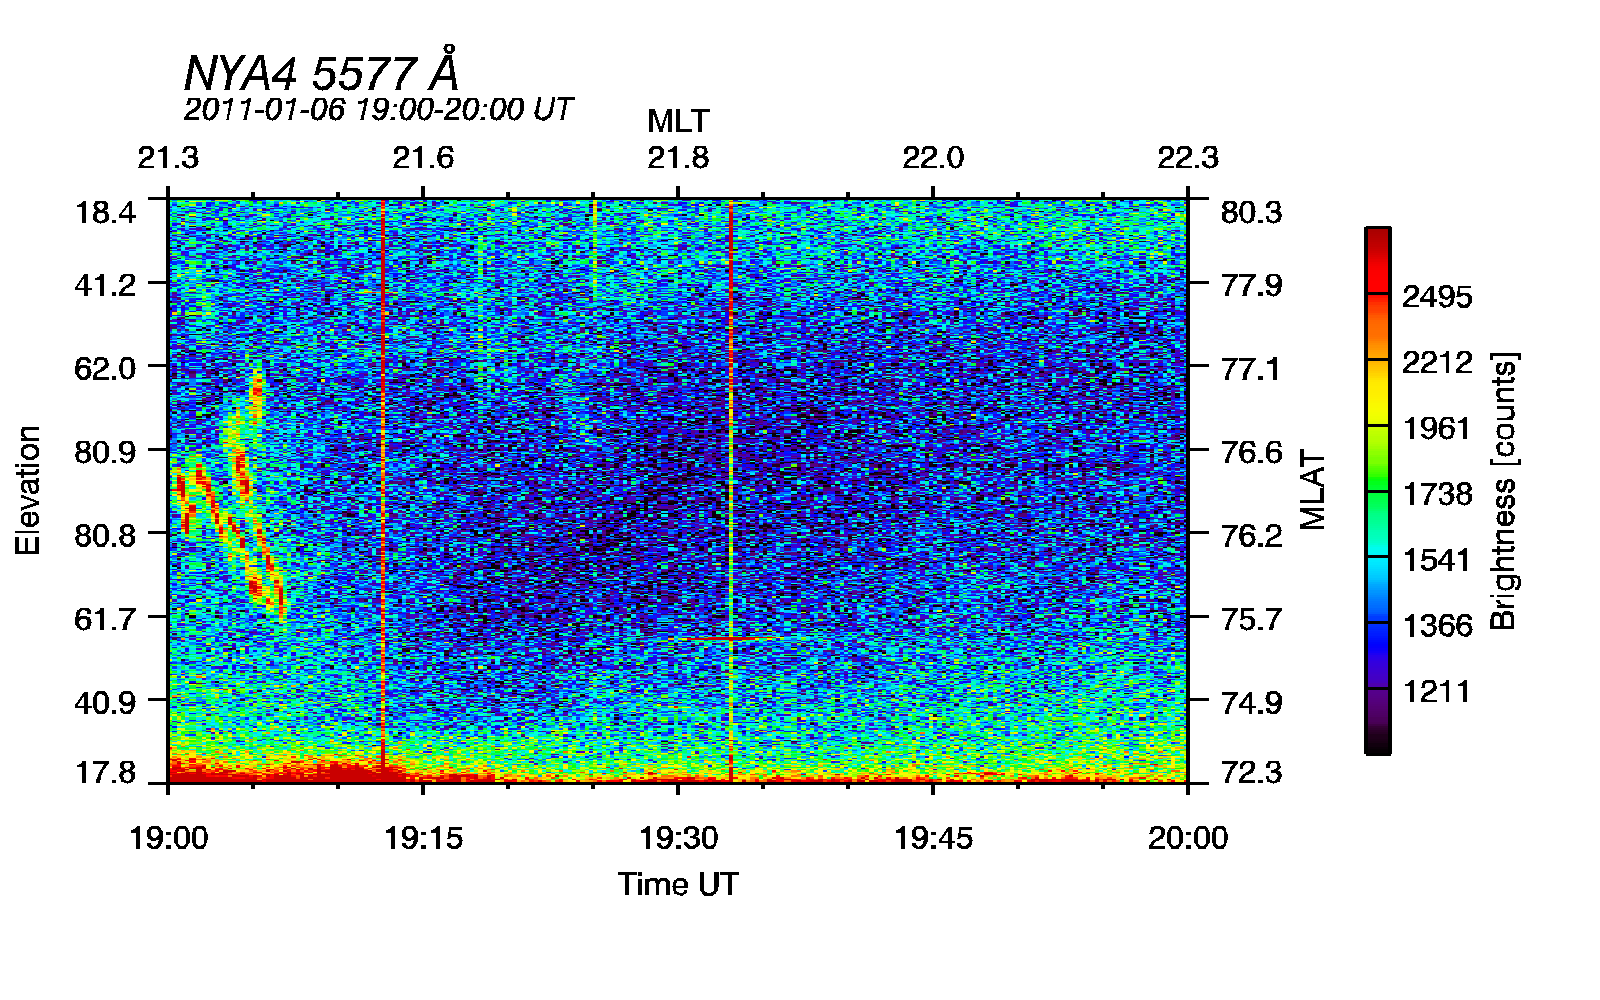
\includegraphics[width=\textwidth]{SvalbardImager5577A19.png}
	\caption{ SvalbardImager at 19:00 UT \label{SBI_5_19}}
\end{subfigure}
\begin{subfigure}{0.3\textwidth}
\centering
	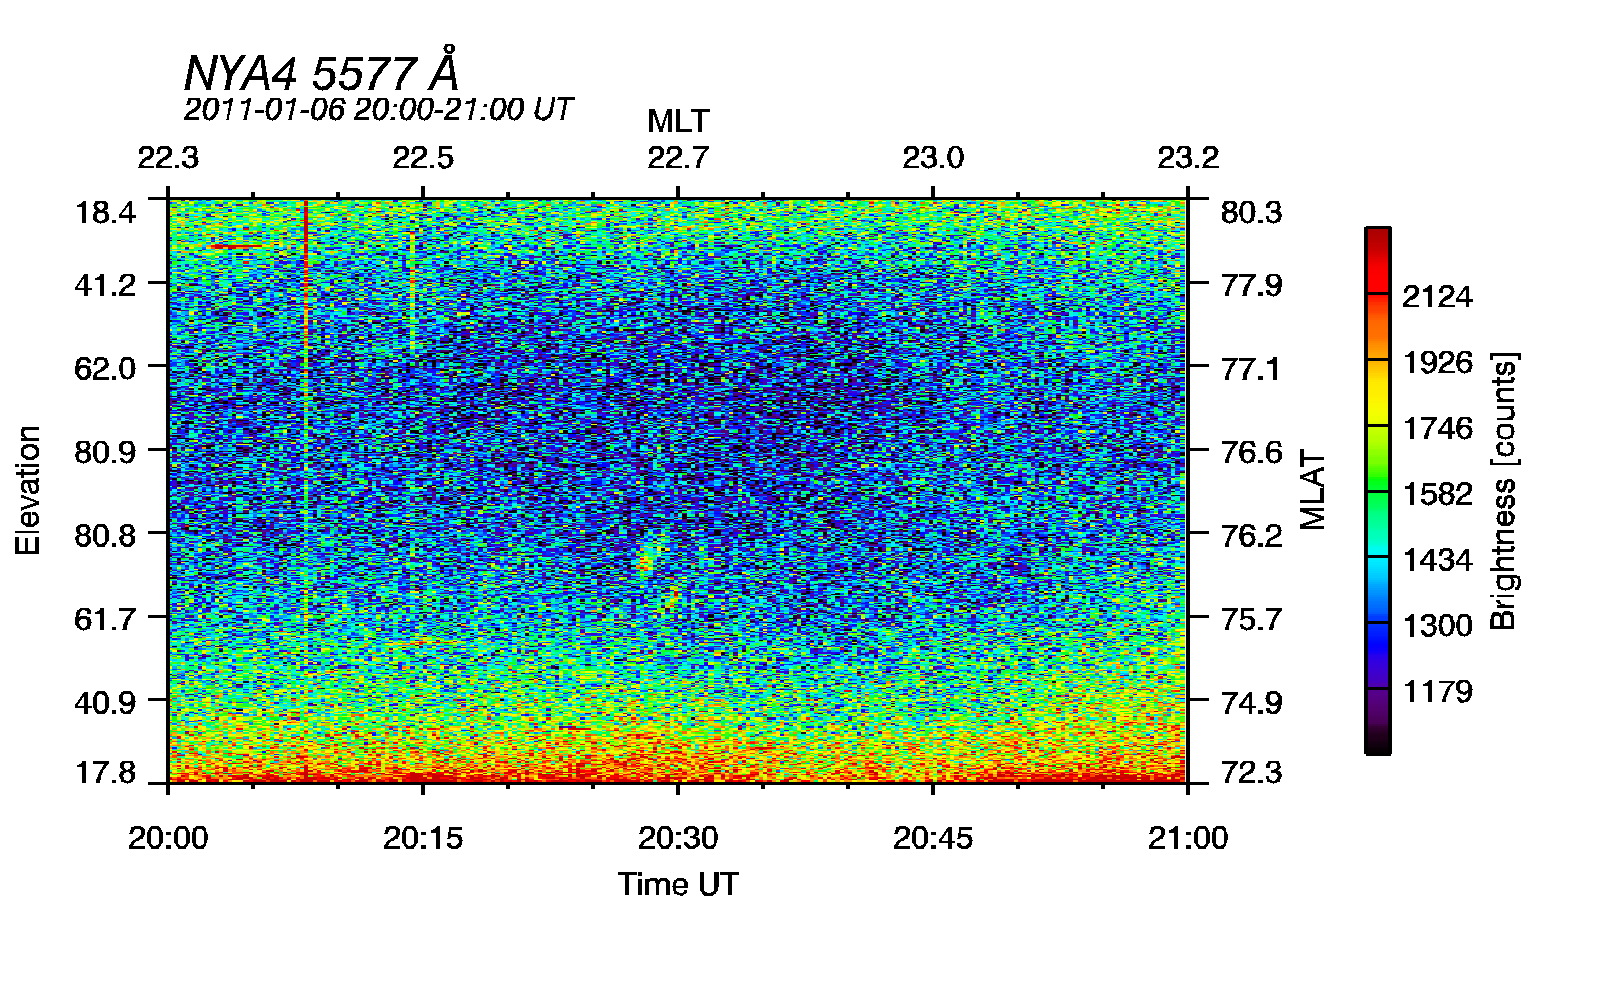
\includegraphics[width=\textwidth]{SvalbardImager5577A20.png}
	\caption{ SvalbardImager at 20:00 UT \label{SBI_5_20}}
\end{subfigure}
\begin{subfigure}{0.3\textwidth}
\centering
	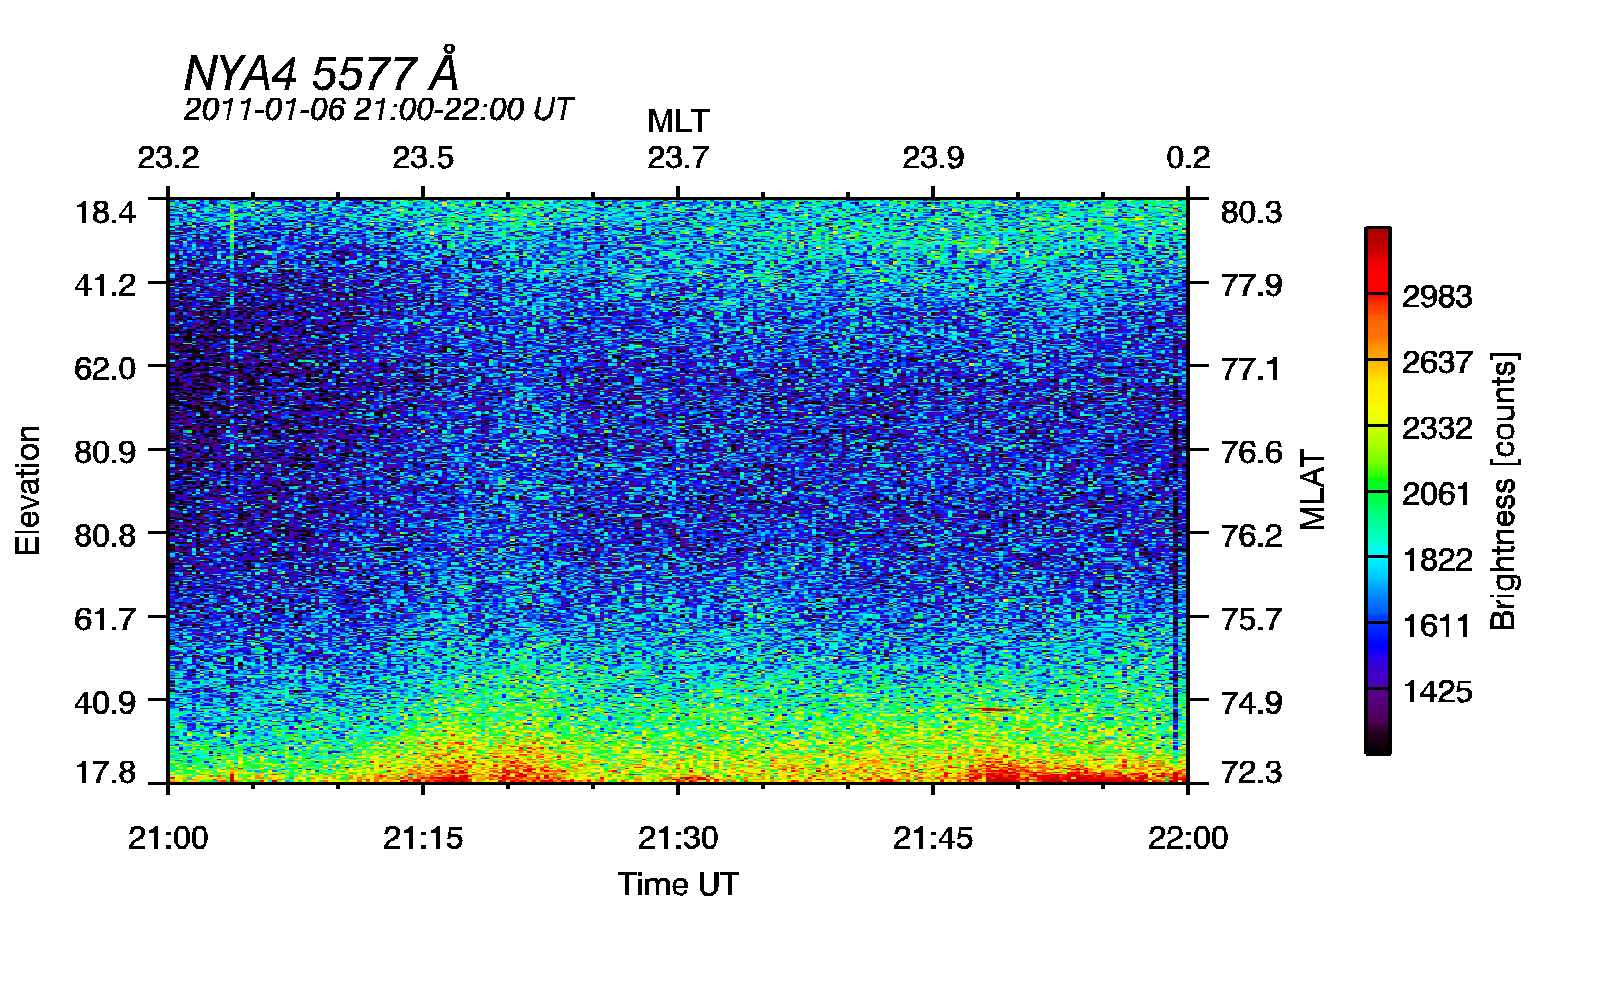
\includegraphics[width=\textwidth]{SvalbardImager5577A21.png}
	\caption{ SvalbardImager at 21:00 UT \label{SBI_5_21}}
\end{subfigure}
\begin{subfigure}{0.3\textwidth}
\centering
	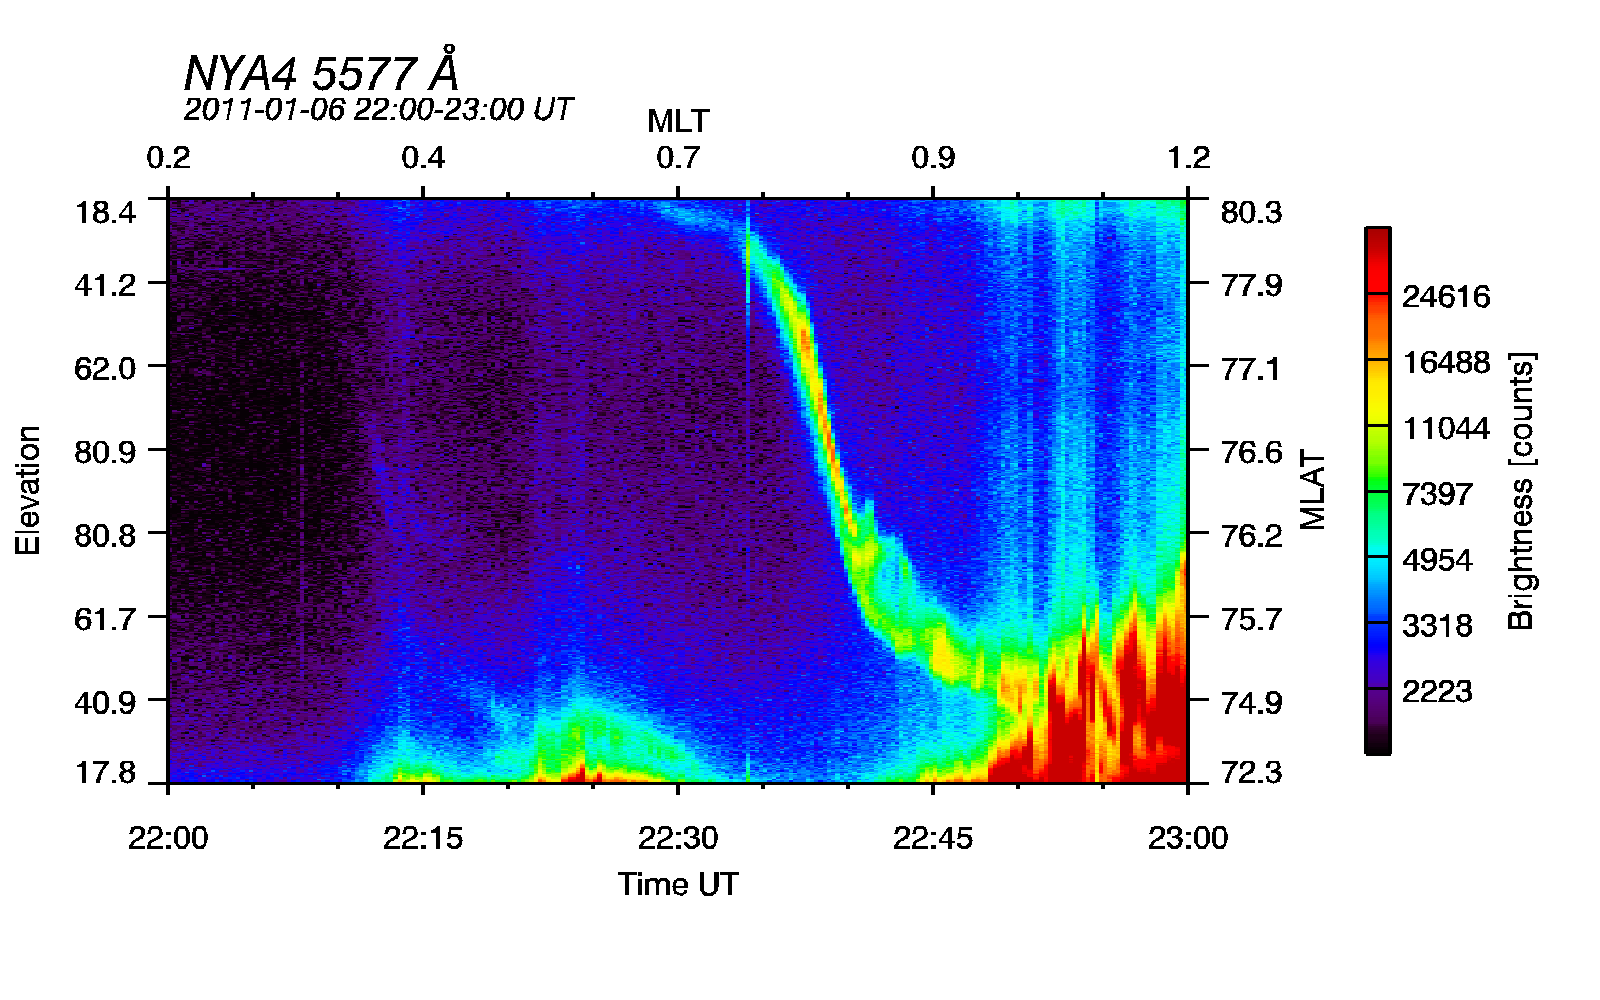
\includegraphics[width=\textwidth]{SvalbardImager5577A22.png}
	\caption{ SvalbardImager at 22:00 UT \label{SBI_5_22}}
\end{subfigure}
\begin{subfigure}{0.3\textwidth}
\centering
	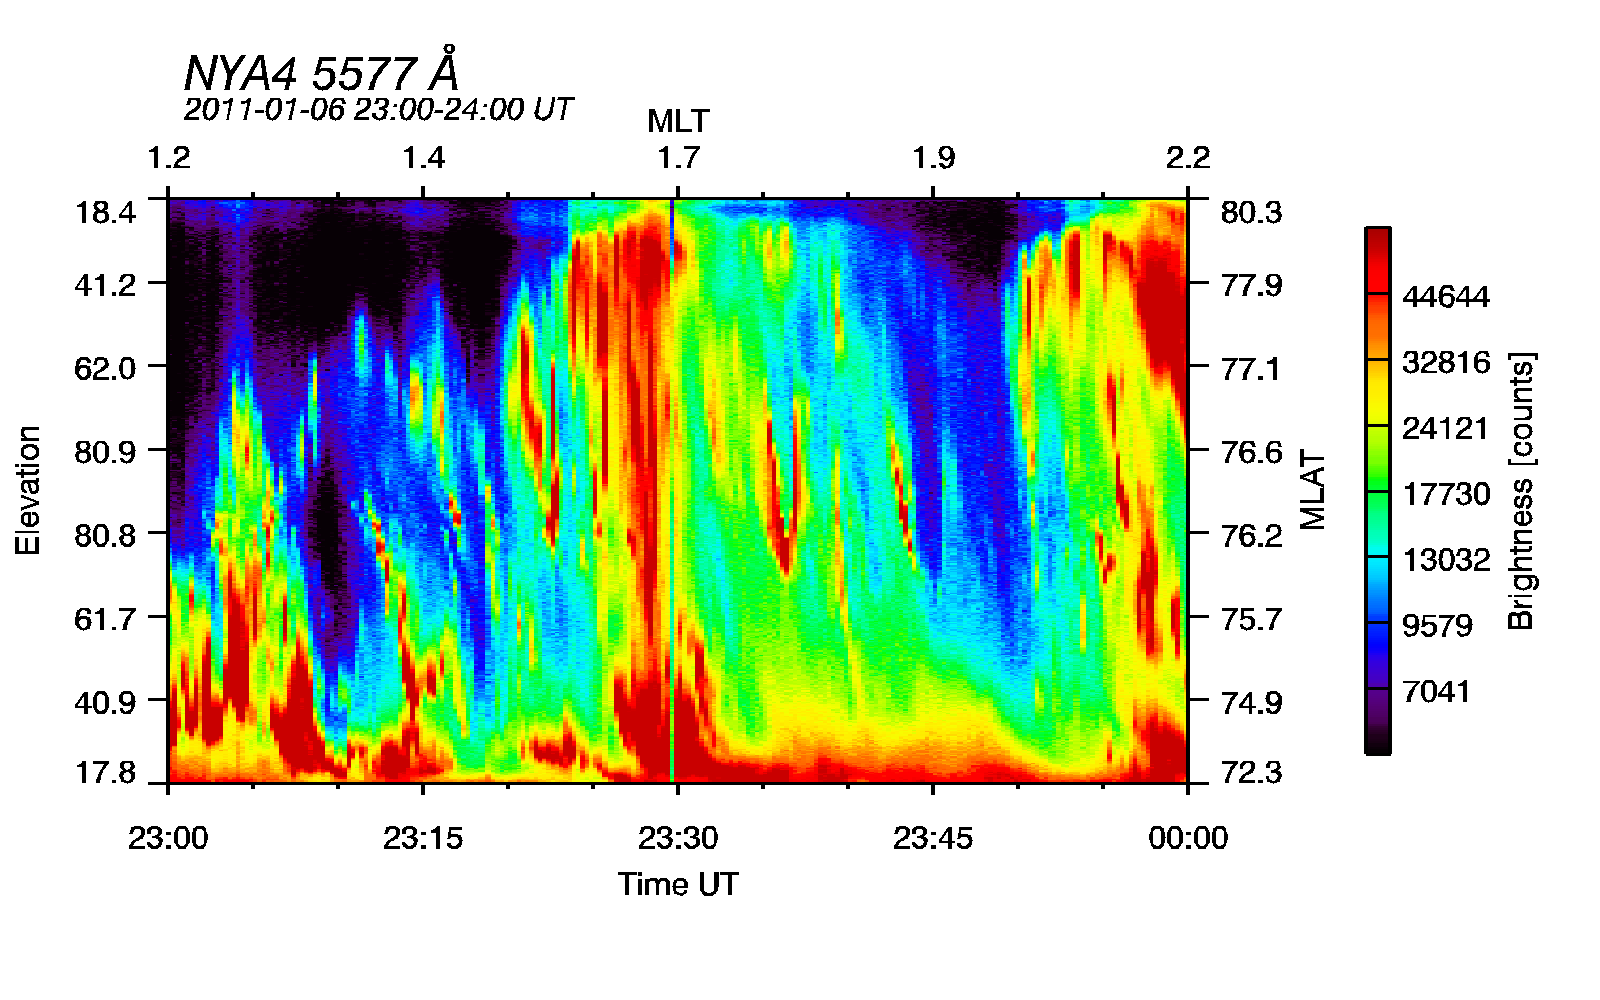
\includegraphics[width=\textwidth]{SvalbardImager5577A23.png}
	\caption{ SvalbardImager at 23:00 UT \label{SBI_5_23}}
\end{subfigure}
\caption{Ketograms from the SvalbardImager for $\lambda=5577 \cdot 10^{-10} \mathrm{m}$, different times }
\label{SBI_5_timedevelop}
\end{figure}
\\
The Svalbard imager for the wavelength of $\lambda=630 nm$ shows qualitatively the same as the imager of $\lambda=577.7 nm$.  This can be seen in figure \ref{SBI_6_timedevelop}. The figures \ref{SBI_6_18} to \ref{SBI_6_23} show each intervals of 1 hour. 
\clearpage


\section{Discussion \label{discussion}}

In this section, we want to explain our observations. We will also try to connect our observation with what we expect from theory. 
It is also very interesting to see, whether the data from the different measurements can be interpreted in a sense-full, physical way.
%ACE- discussion

The Dungey cycle, auroral substorms and the twin-cell convection are all dependent on the IMF. Especially the sign of the $B_z$-component is really important because it determines, whether magnetic reconnection occurs or not. (compare \ref{_CHAP_THEO_Dungey cycle}) Therefore, it makes sense to look first at the data from ACE. 
If we assume that the solar wind needs on average 1 hour to travel from ACE to Earth, we can say that the $B_z$-component is positive from 19:00 UT to 21:15 UT at Earth's position. At approximately 21:15 UT, the negative turn of the IMF reaches the Earth. While the $B_z$ component is negative, we expect that magnetic reconnection on dayside happens. When magnetic reconnection on dayside occurs, open magnetic flux is added to the polar cap. If magnetic reconnection on the nightside doesn't take place, the polar cap should grow. We assume that the rate of magnetic reconnection at far Earth neutral line is low. 
Southward orientation of the IMF is needed in order to enter the growth phase of a substorm. During the growth phase, magnetic energy is stored in the tail. This energy can later be released through a substorm. On average, we observed a southward orientation of the magnetic field until 01:45 UT of the 7th of January 2011. However, we can see a sudden peak in the $B_z$ component at 22:20 UT at Earth. This sudden turn of the IMF might lead to what we call polar arcs, which are aurora that moves from the very high latitudes then southward towards the polar cap. Research suggest that these arcs might be somehow connected to auroral substorms, and that they are more prominent in times of northward IMF \cite{paper3}. We do not know which type of polar arc this might be, as there are different types with specific characteristics, some of the different types are reviewed in \cite{paper4}. 
%Groundbasedmagnetometer- discussion

Next, we want to look for signs of a substorm. A good method to detect substorms is to look at the data from the ground-based-magnetometers. A substorm normally leads to westward electro-jets, which lead to a magnetic field according to Amperes law. In the end, if a substorm kicks in, this leads to a depression of the south-north component of the magnetic field measured on the ground. A eastward eletrojet would lead to a increase of the south-north component of the magnetic field measured on the ground. We now have a look at the data from \ref{0_CHAPTER_AMPERE}. As described there, we can see a depression of the south-north component of the magnetic field at approximately 22:00 UT. The depression reaches a minimum at approximately 22:30 UT. (depending on the specific station) This depression is a strong hint to a substorm happening in between 22:00 UT and 23:00 UT. 
At the stations more southward, you can see that there is first an increase of the south-north-magnetic field and then a depression. The most likely interpretation is that there is a local current flowing eastward, which leads to an increase of the magnetic field. Depending on the position of the station and other parameters, eastward electrojets can be measured. This depends also on the shape of the twin cell convection at the specific time. An important parameter to look at would be the $B_y$-component of the IMF at this time because this determines the specific shape of the twin cell convection. For further research on this, you can have a look in paper \cite{paper2}.
% KOMENTAR: Not finished yet

% Superdarn
Furthermore, we want to have a look at the data from SuperDARN. (see chapter \ref{0_CHAPTER_SUPERDARN}) We notice, that the shape of the electric potential fits the theoretical predictions. We can see two cells, which can be characterized through a region with negative electric potential (blue) and a region with positive electric potential (red). In the region with negative electric potential, the charged particles move clockwise and in the positive region the particles move anti-clockwise. 
Also the orientation of the two cells fit. The direction to the Sun is in the figures \ref{Super_overview} at noon.
The twin cells should be separated by a line from approximately  noon to midnight. (directions) This depends also on the components of the IMF. The orientation of the twin cells seems to be right.  
Looking at the time development of the electric field, we can now connect the increase of the electric potential from 21:00 UT to 22:00 UT with other physical phenomena. 
From section \ref{0_CHAPTER_ACE}, we know that the negative turn of the $B_z$ component of the IMF is at about 21:45 UT on Earth. A southward IMF results in magnetic reconnection on dayside. Magnetic reconnection on the dayside is directly coupled to the twin-cell convection pattern. The twin cell convection should increase, which is exactly what we can see in the data. From the Ground-based magnetometer, we got a strong  hint of an auroral substorm kicking in between 22:00 UT and 23:00 UT. Substorms decrease the total magnetic flux in the polar cap. We can see that from 22:00 UT to 23:00 UT, that $\phi_{pc}$ stays approximately constant.
All in all, we can say that the theory matches the experimental data concerning this measurement.\\ 
% Ampere discussion 
We want now to discuss the data from the Measurement AMPERE.(observations described in chapter \ref{0_CHAPTER_AMPERE}) The  curl of the magnetic field measured parallel 
to the surface of Earth determines the current flow perpendicular to the surface to Earth. The field aligned currents are coupled to the Dungey cycle. To be more precise, The hall currents are driven by the Dungey cycle. The hall currents lead to a electric field at a specific altitude. Pedersen currents (mostly ions) follow this electric field. The pederson currents are not source free. At the spots, where it comes to a accumulation of charge, we expect field aligned currents to close this current system. Depending on the sign of the accumulated charge, the field aligned currents flow into space or in the direction of Earth's surface. 
Derived from this idea, we expect region 1 and region 2 currents. Both can be seen in the data. Since the field aligned currents are as described in chapter \ref{_CHAP_THEO_currentsystem earth} coupled to the twin cell convection, we expect also an increase of FAC when twin cell convection increases. The data support this argument since we can see an increase of FAC from 21:00 UT to 24:00 UT , which fits to the development of the twin cell convection. 
This means that we have qualitatively a good match between theory matches and experiment.
%KOMENTAR: What determines the strength of the Field aligned currents?

% Svalbardimager- discussion
Finally, let us look at the Svalbard-imager. The first significant development in the imager can be seen at approximately 22:35 UT. A small brightened area moves equator-ward and westward. We could not relate the movement of the auroral arc to a specific physical phenomena, but it seems to trigger the onset of the first substorm. At 22:45 UT, we can see an increase in intensity of both wavelength for lower latitudes. This seems to be the first substorm detected this night. The time of the substorm seems to be reasonable. In the time before the substorm, we know from the data gathered from ACE that the $B_z$ component on the IMF was negative from 22:15 UT on. In this time, energy should have been stored in the magnetotail of Earth by adding magnetic flux. 
From reference \cite{Buch2}[p.419, Fig. 13.14.], we know that "sudden changes in the solar-wind dynamic pressure and, more frequently, northward turnings of the IMF can trigger the sudden unloading of stored energy". At approximately 22:20 UT, the IMF-$B_z$-component on Earth turns suddenly northward and southward again. It is possible that this sudden change triggered the onset of the substorm. In the time after 23:00 UT, we can see several timeslots of 5-10 minutes each, where we measure high light intensity. One peaks around 23:15 UT, one peaks at 23:30 UT and the last one peaks about 24:00 UT. In between, we see a significant loss of intensity. 
This can be interpreted as several substorms happening in pulses. 

\section{Conclusion}

The aim of our project is to study ionospheric and auroral dynamics in response in solar wind conditions. We will study for example the twin cell convection, field aligned currents, pedersen currents and auroral activity and their relation to the IMF. 
The average behaviour of the system can be described for large time scales with the Dungey cycle. On top of this cycle, we took substorms under consideration. Substorms are important because they release stored magnetic energy from the tail through magnetic reconnection. Substorms contribute a lot to sudden brightening. 
We found out that the $B_z$-component of the IMF plays indeed a big role for the whole system. 


\newpage
\section{Additional plots}

\begin{figure}[h]
\centering
\begin{subfigure}{0.3\textwidth}
\centering
	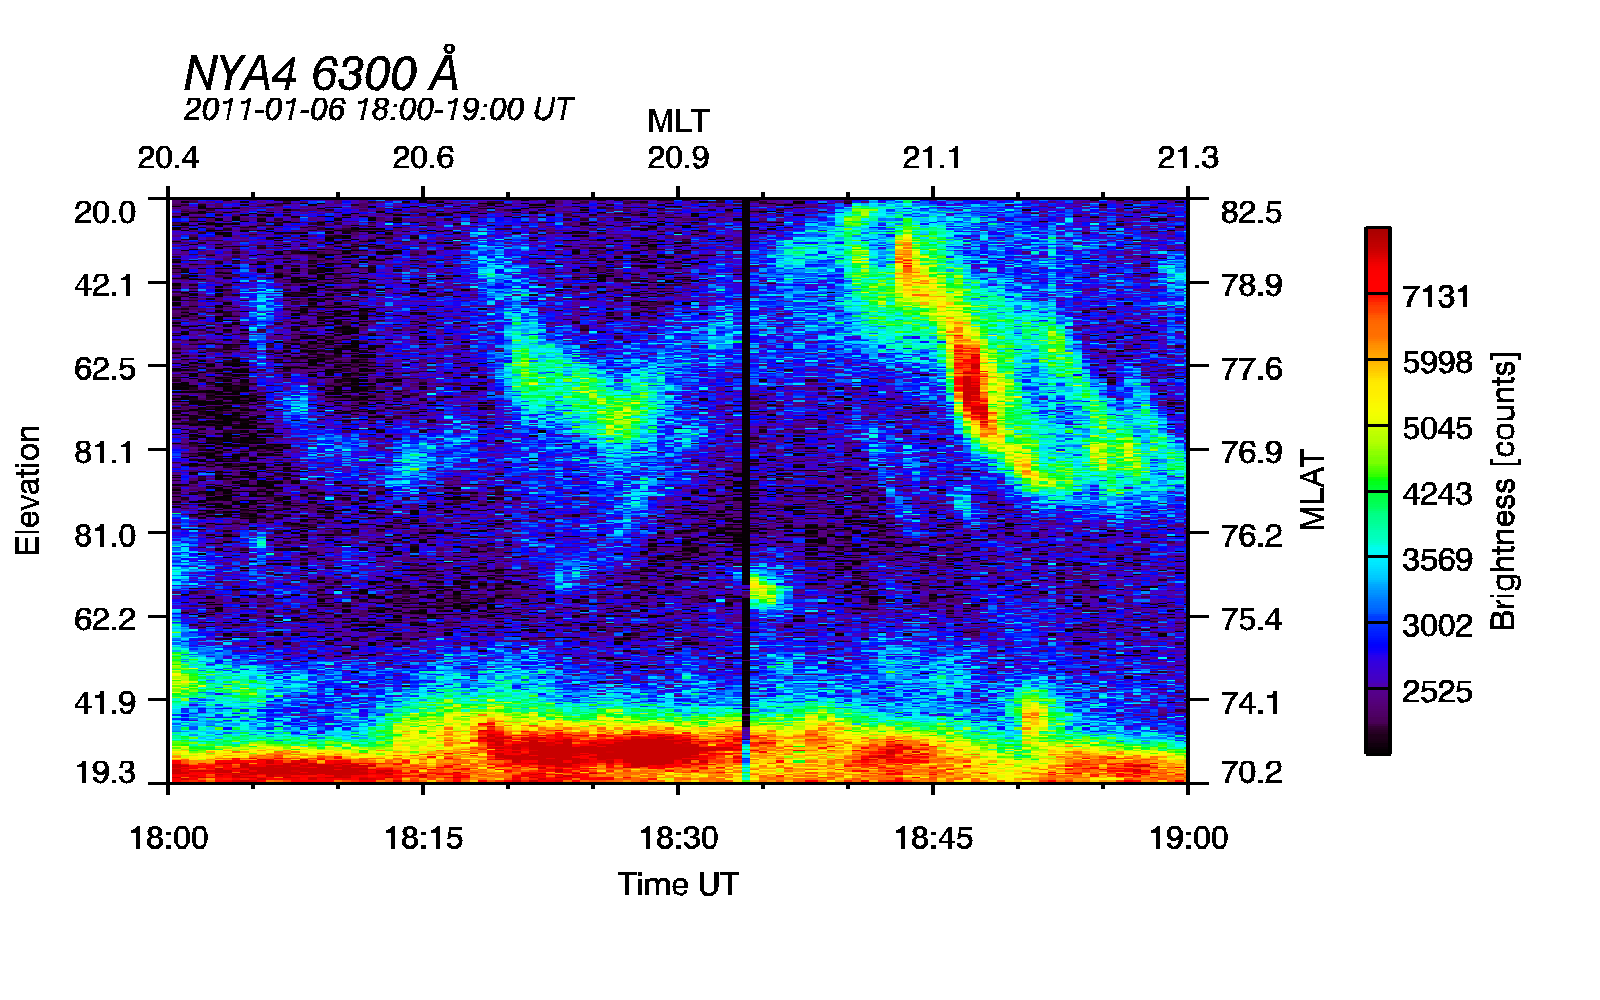
\includegraphics[width=\textwidth]{SvalbardImager6300A18.png}
	\caption{ SvalbardImager at 18:00 UT \label{SBI_6_18}}
\end{subfigure}
\begin{subfigure}{0.3\textwidth}
\centering
	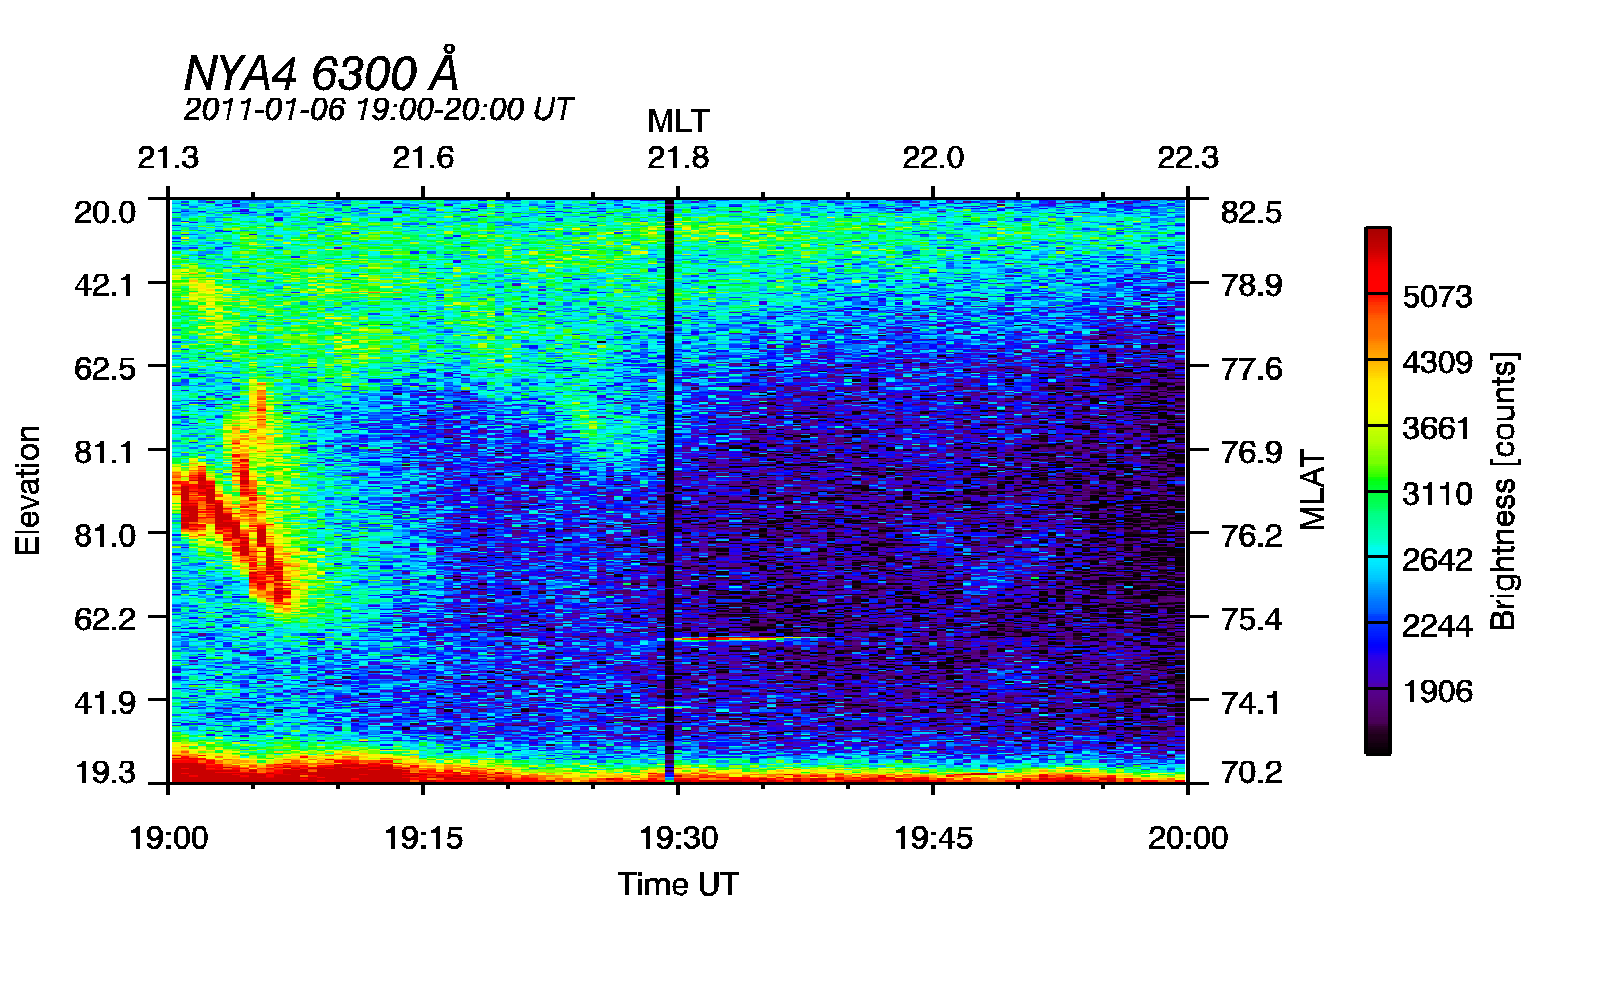
\includegraphics[width=\textwidth]{SvalbardImager6300A19.png}
	\caption{ SvalbardImager at 19:00 UT \label{SBI_6_19}}
\end{subfigure}
\begin{subfigure}{0.3\textwidth}
\centering
	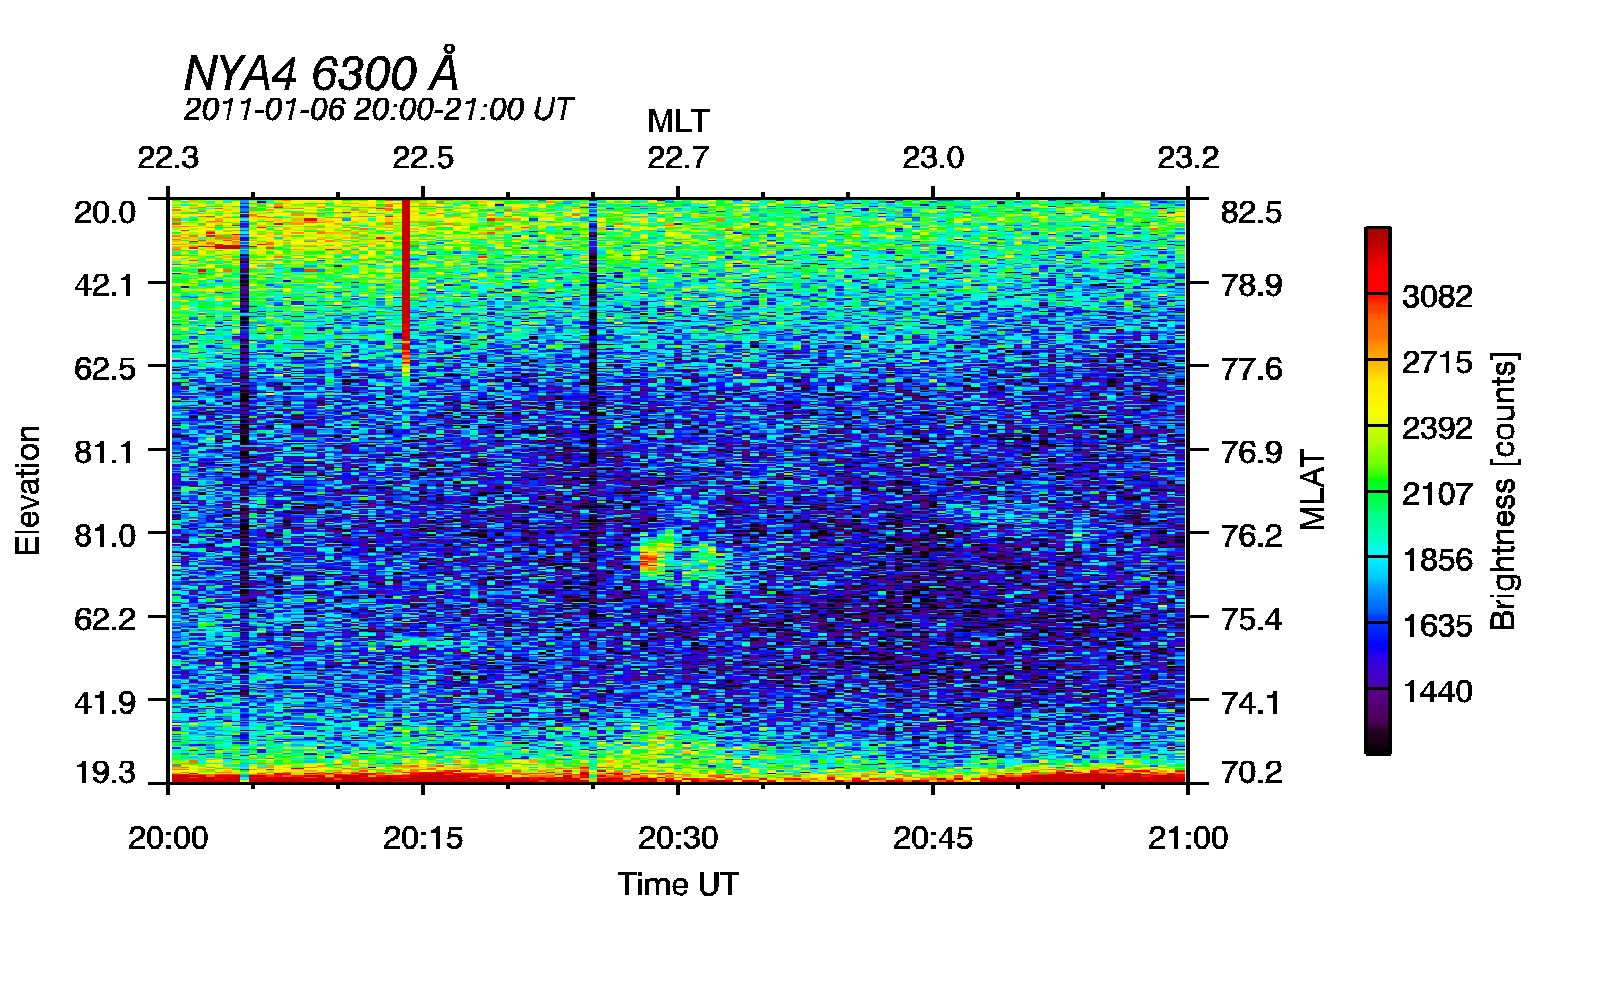
\includegraphics[width=\textwidth]{SvalbardImager6300A20.png}
	\caption{ SvalbardImager at 20:00 UT \label{SBI_6_20}}
\end{subfigure}
\begin{subfigure}{0.3\textwidth}
\centering
	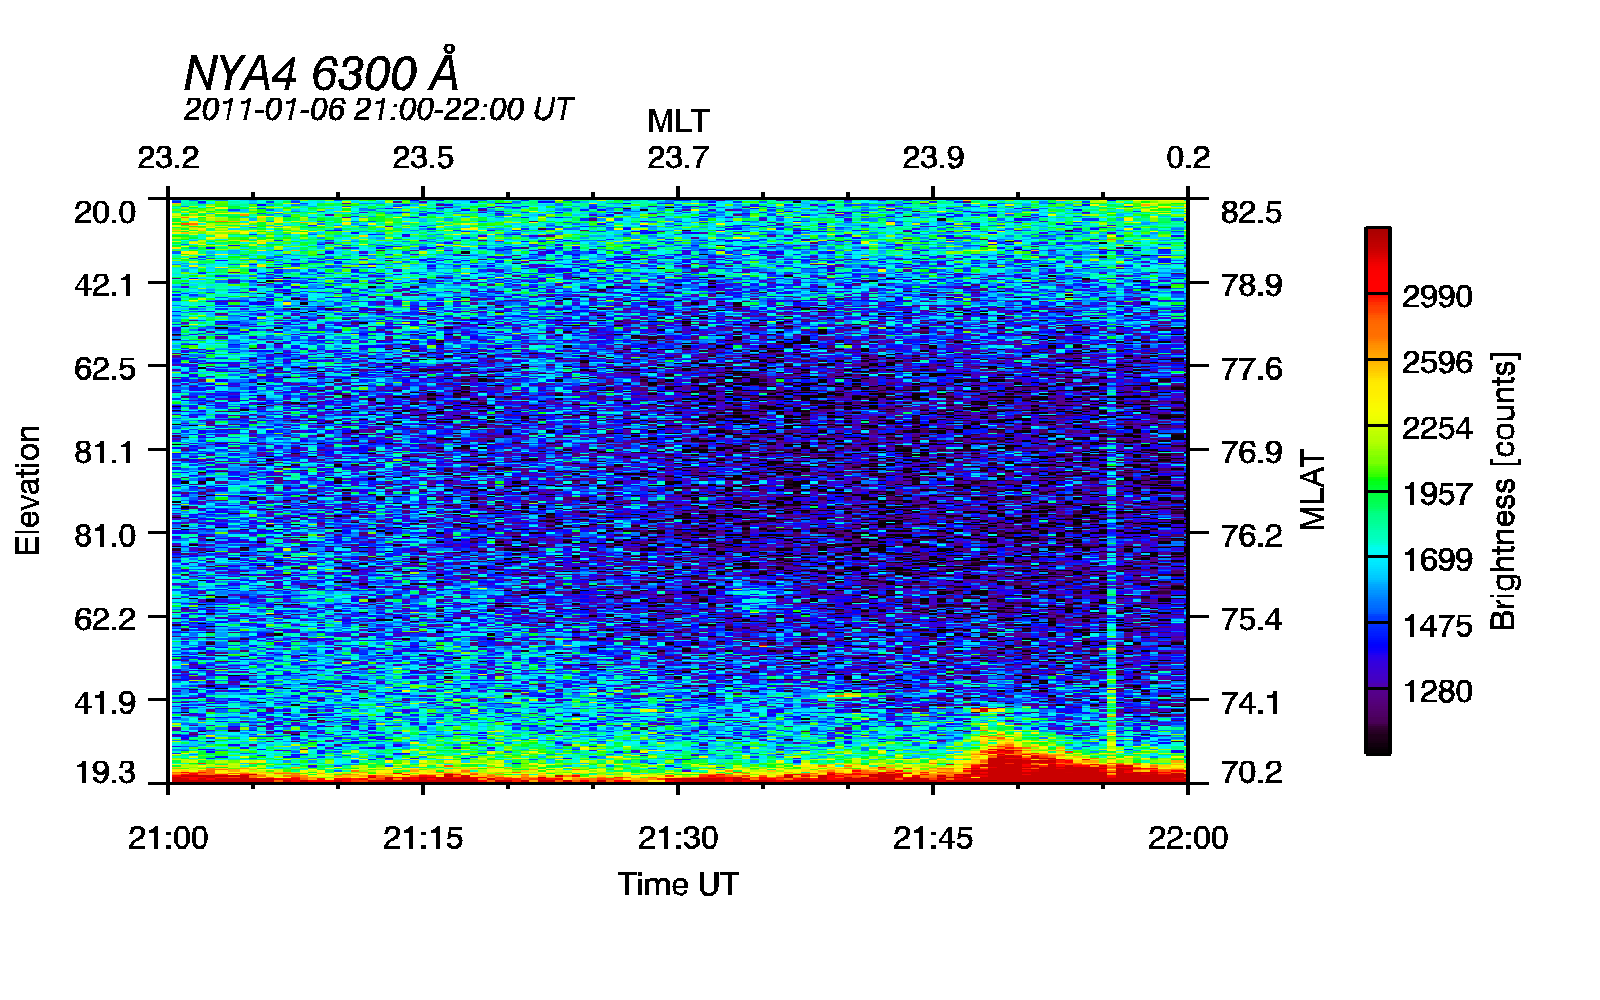
\includegraphics[width=\textwidth]{SvalbardImager6300A21.png}
	\caption{ SvalbardImager at 21:00 UT \label{SBI_6_21}}
\end{subfigure}
\begin{subfigure}{0.3\textwidth}
\centering
		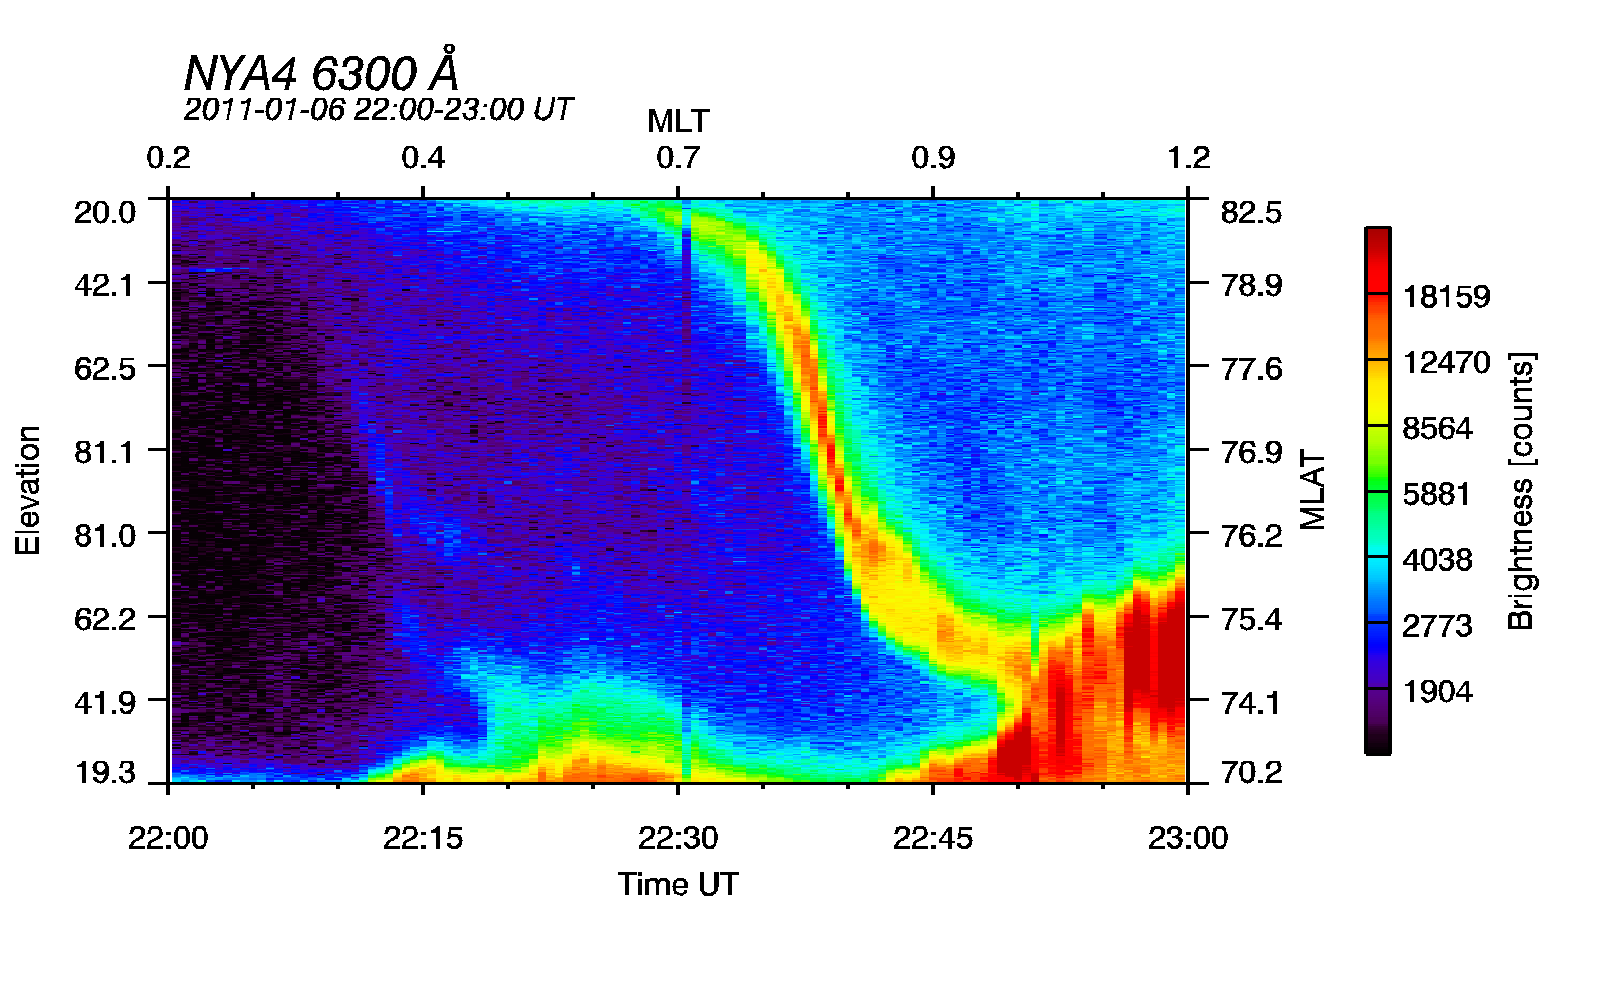
\includegraphics[width=\textwidth]{SvalbardImager6300A22.png}
	\caption{ SvalbardImager at 22:00 UT \label{SBI_6_22}}
\end{subfigure}
\begin{subfigure}{0.3\textwidth}
\centering
	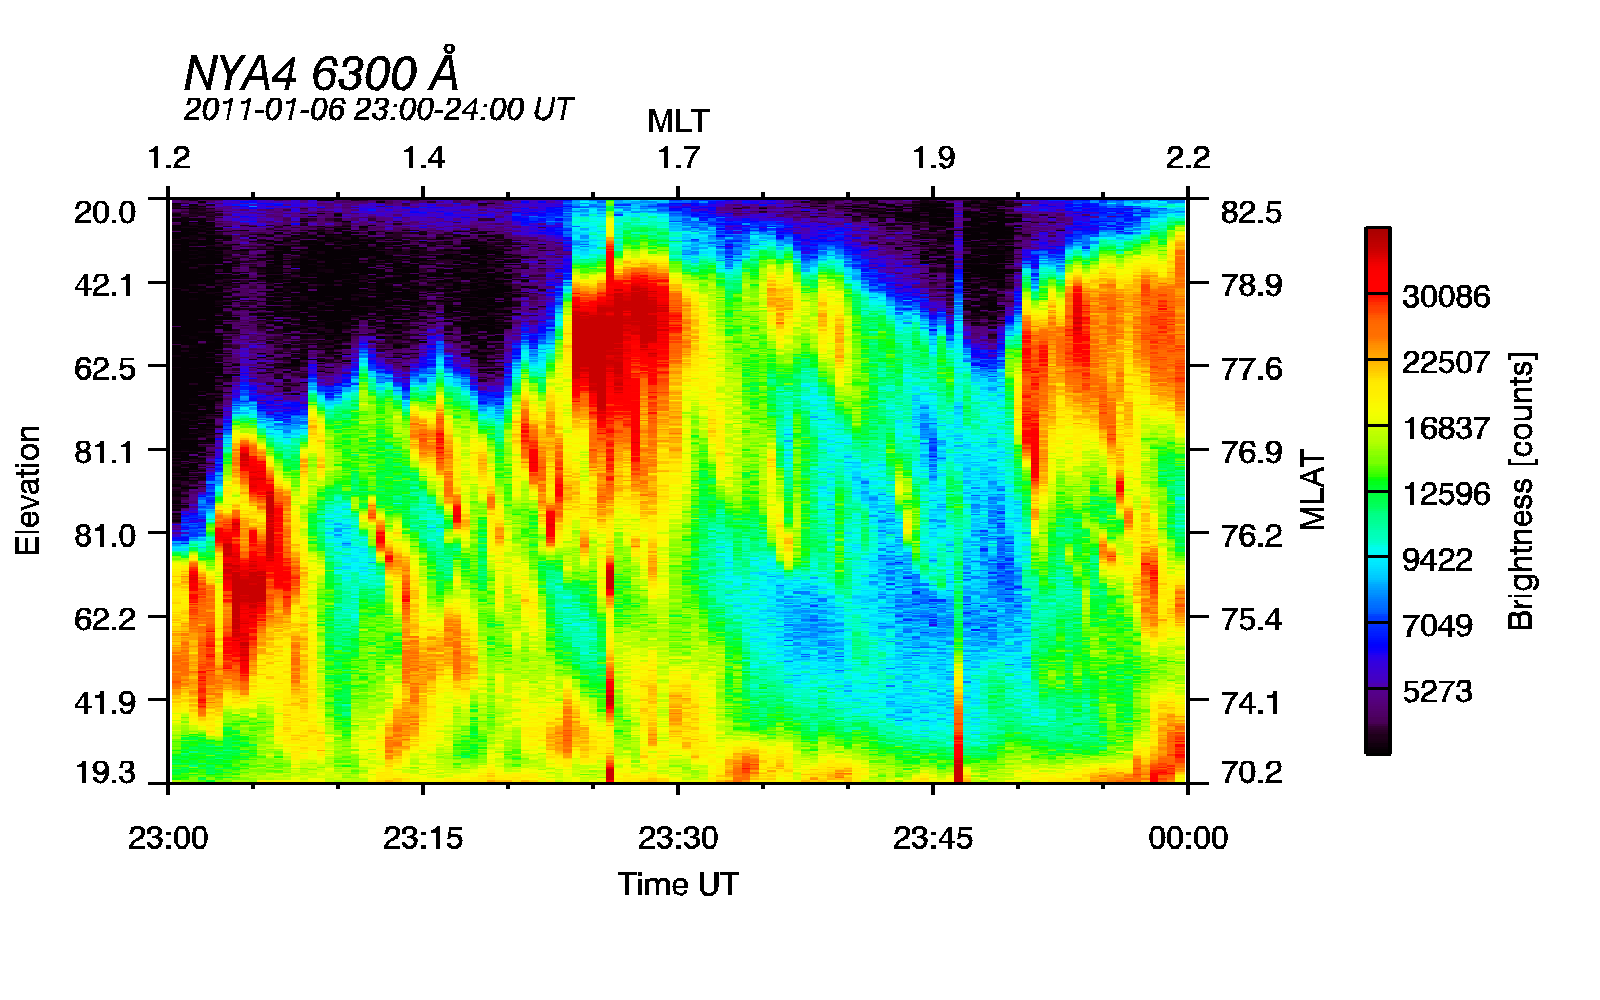
\includegraphics[width=\textwidth]{SvalbardImager6300A23.png}
	\caption{ SvalbardImager at 23:00 UT \label{SBI_6_23}}
\end{subfigure}
\caption{Ketograms from the SvalbardImager for $\lambda=6300 \cdot 10^{-10} \mathrm{m}$, different times }
\label{SBI_6_timedevelop}
\end{figure}

\begin{figure}[h]
\centering
\caption{Map of the stations used for Groundbasedmagnetometers}
\label{Groungbasedmagnetometers_maps}
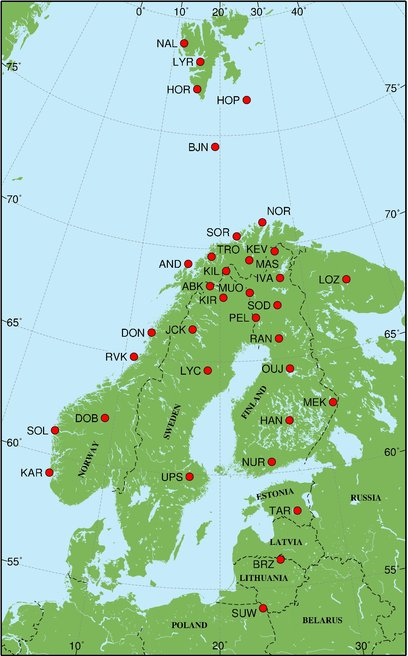
\includegraphics[width=0.3\textwidth]{Stations.jpg}
\end{figure}

\clearpage


\begin{thebibliography}{mustermarke}
\bibitem[1]{Link1} \url{http://www.windows2universe.org/earth/Magnetosphere/tour/tour_earth_magnetosphere_07.html&edu=high}, 27.11.2015
\bibitem[2]{Link2} \url{http://www.nasa.gov/mission_pages/sunearth/news/ace-15th.html}, 27.11.2015
\bibitem[3]{Buch} Gerd W. Prölss: Physics of the Earth's Space Environment (An Introduction).Bonn  dec 2003 
\bibitem[4]{paper1} S.-I. Akasofu ; The development of the auroral substorm; Planetary and Space Science; Volume 12, Issue 4, April 1964, Pages 273-282
\bibitem[5]{paper2} Ruohoniemi, J. M., R. A. Greenwald, Dependencies of high-latitude plasma convection: Consideration of interplanetary magnetic field, seasonal and universal time factors in statistical patterns, J. Geophys.
Res., 110, A09204, doi:10.1029/2004JA010815, 2005.
\bibitem[6]{Buch2} Kievelson and Russel, Introduction to Space Physics, Chapters 9, 13, and 14
\bibitem[7]{Buch3} Baumjohann, Treumann, Basic Space Plasma Physics, 1996 by Imperial College Press
\bibitem[8]{paper3} J.S. Murphree, J.B. Austin, D.J. Hearn, L.L. Cogger, R.D. Elphinstone, J. Woch Satellite observations of polar arcs, J. Atmospheric and Terrestrial Physics
Volume 56, Issue 2, February 1994, Pages 265–284
\bibitem[9]{paper4}     L. Zhu, R.W. Schunk, J.J. Sojka, Polar cap arcs: a review, Revised 15 July 1996, Accepted 2 August 1996, Available online 5 June 1998, Page 8
\end{thebibliography}
\end{document}